

\documentclass{beamer}
\usepackage[utf8]{inputenc}
\usepackage{graphicx}
% Replace the \documentclass declaration above
% with the following two lines to typeset your 
% lecture notes as a handout:
%\documentclass{article}
%\usepackage{beamerarticle}


% There are many different themes available for Beamer. A comprehensive
% list with examples is given here:
% http://deic.uab.es/~iblanes/beamer_gallery/index_by_theme.html
% You can uncomment the themes below if you would like to use a different
% one:
%\usetheme{AnnArbor}
%\usetheme{Antibes}
%\usetheme{Bergen}
%\usetheme{Berkeley}
%\usetheme{Berlin}
%\usetheme{Boadilla}
%\usetheme{boxes}
%\usetheme{CambridgeUS}
%\usetheme{Copenhagen}
%\usetheme{Darmstadt}
%\usetheme{default}
%\usetheme{Frankfurt}
\usetheme{Goettingen}
%\usetheme{Hannover}
%\usetheme{Ilmenau}
%\usetheme{JuanLesPins}
%\usetheme{Luebeck}
%\usetheme{Madrid}
%\usetheme{Malmoe}
%\usetheme{Marburg}
%\usetheme{Montpellier}
%\usetheme{PaloAlto}
%\usetheme{Pittsburgh}
%\usetheme{Rochester}
%\usetheme{Singapore}
%\usetheme{Szeged}
%\usetheme{Warsaw}

\title{Instalación de requerimientos de trabajo}

% A subtitle is optional and this may be deleted
\subtitle{Unity, Android Studio y JDK}

\author{Yas\inst{1} \and Rocío\inst{2}}
% - Give the names in the same order as the appear in the paper.
% - Use the \inst{?} command only if the authors have different
%   affiliation.

\institute[Universities of Somewhere and Elsewhere] % (optional, but mostly needed)
{
  \inst{1}%
  Instituto Politécnico Nacional
  \and
  \inst{2}%
  Escuela Superior de Cómputo}
% - Use the \inst command only if there are several affiliations.
% - Keep it simple, no one is interested in your street address.

\date{Documentación, 2017}
% - Either use conference name or its abbreviation.
% - Not really informative to the audience, more for people (including
%   yourself) who are reading the slides online

\subject{Theoretical Computer Science}
% This is only inserted into the PDF information catalog. Can be left
% out. 

% If you have a file called "university-logo-filename.xxx", where xxx
% is a graphic format that can be processed by latex or pdflatex,
% resp., then you can add a logo as follows:

% \pgfdeclareimage[height=0.5cm]{university-logo}{university-logo-filename}
% \logo{\pgfuseimage{university-logo}}

% Delete this, if you do not want the table of contents to pop up at
% the beginning of each subsection:
\AtBeginSubsection[]
{
  \begin{frame}<beamer>{Outline}
    \tableofcontents[currentsection,currentsubsection]
  \end{frame}
}

% Let's get started
\begin{document}

\begin{frame}
  \titlepage
\end{frame}

\begin{frame}{Índice}
  \tableofcontents
  % You might wish to add the option [pausesections]
\end{frame}

% Section and subsections will appear in the presentation overview
% and table of contents.
\section{Características previas a instalar}

\subsection{Requerimientos mínimos}

\begin{frame}{01}{Optional Subtitle}
  \begin{itemize}
  \item {
    Nos dirigimos a la página oficial de Unity:
    https://store.unity.com/es
  }
  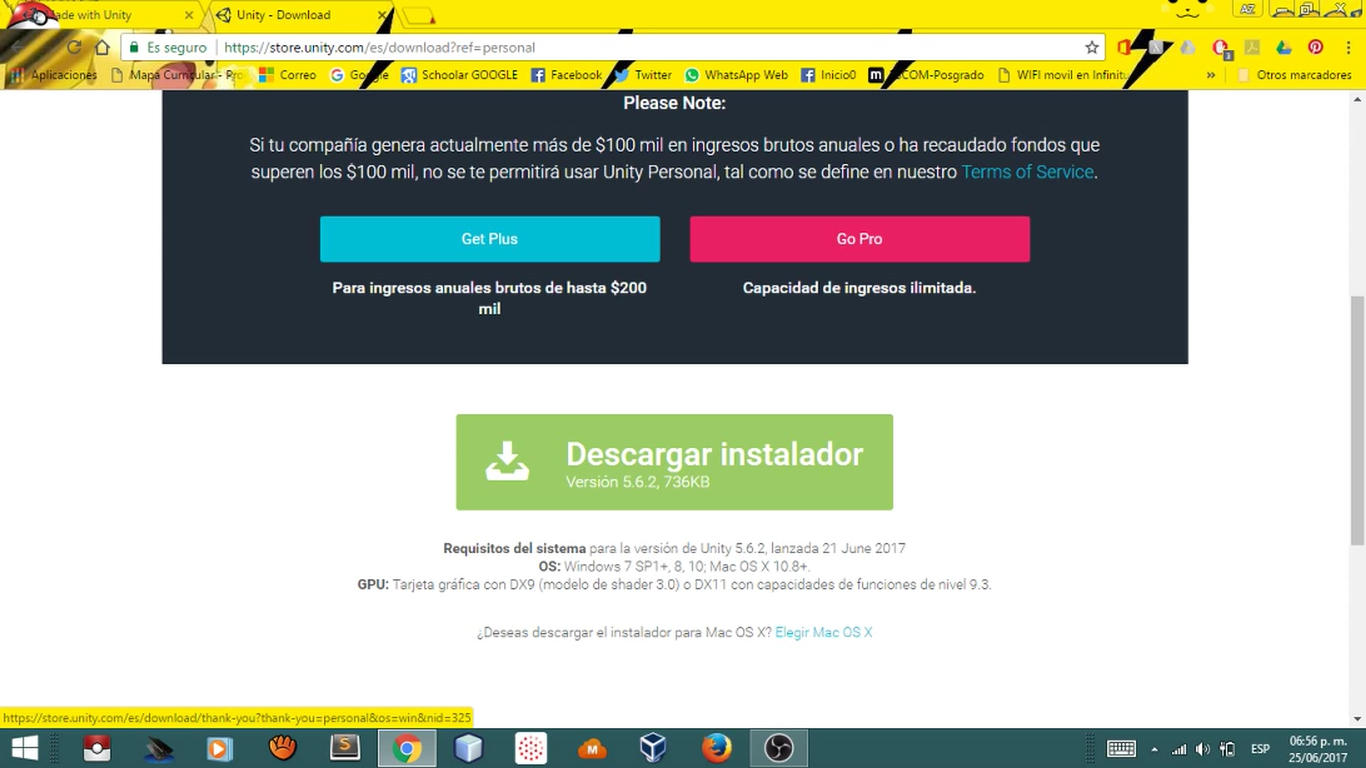
\includegraphics[width=\linewidth]{image/IU01}
  \end{itemize}
\end{frame}

\subsection{Lap Rocío}

\begin{frame}{01}{Optional Subtitle}
  \begin{itemize}
  \item {
    Nos dirigimos a la página oficial de Unity:
    https://store.unity.com/es
  }
  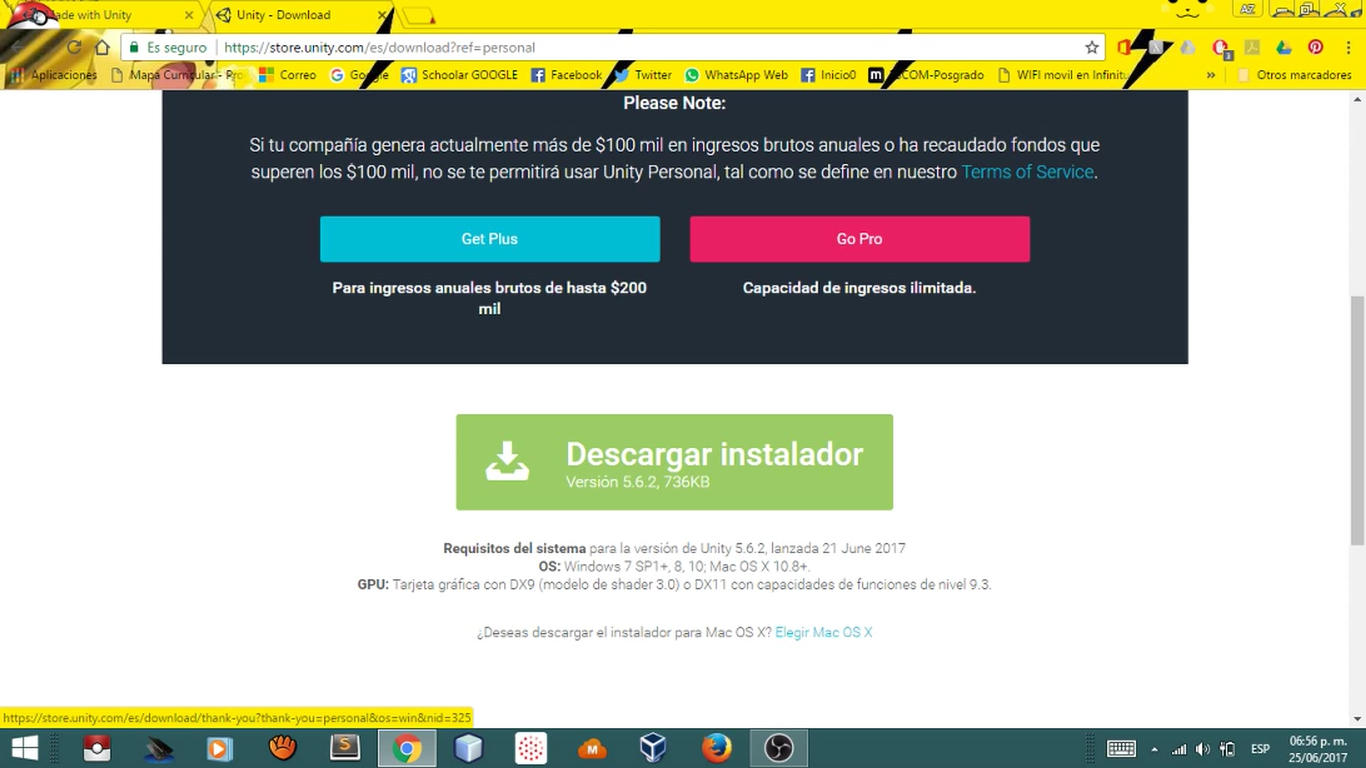
\includegraphics[width=\linewidth]{image/IU01}
  \end{itemize}
\end{frame}

\subsection{Lap Yas}

\begin{frame}{01}{Optional Subtitle}
  \begin{itemize}
  \item {
    Nos dirigimos a la página oficial de Unity:
    https://store.unity.com/es
  }
  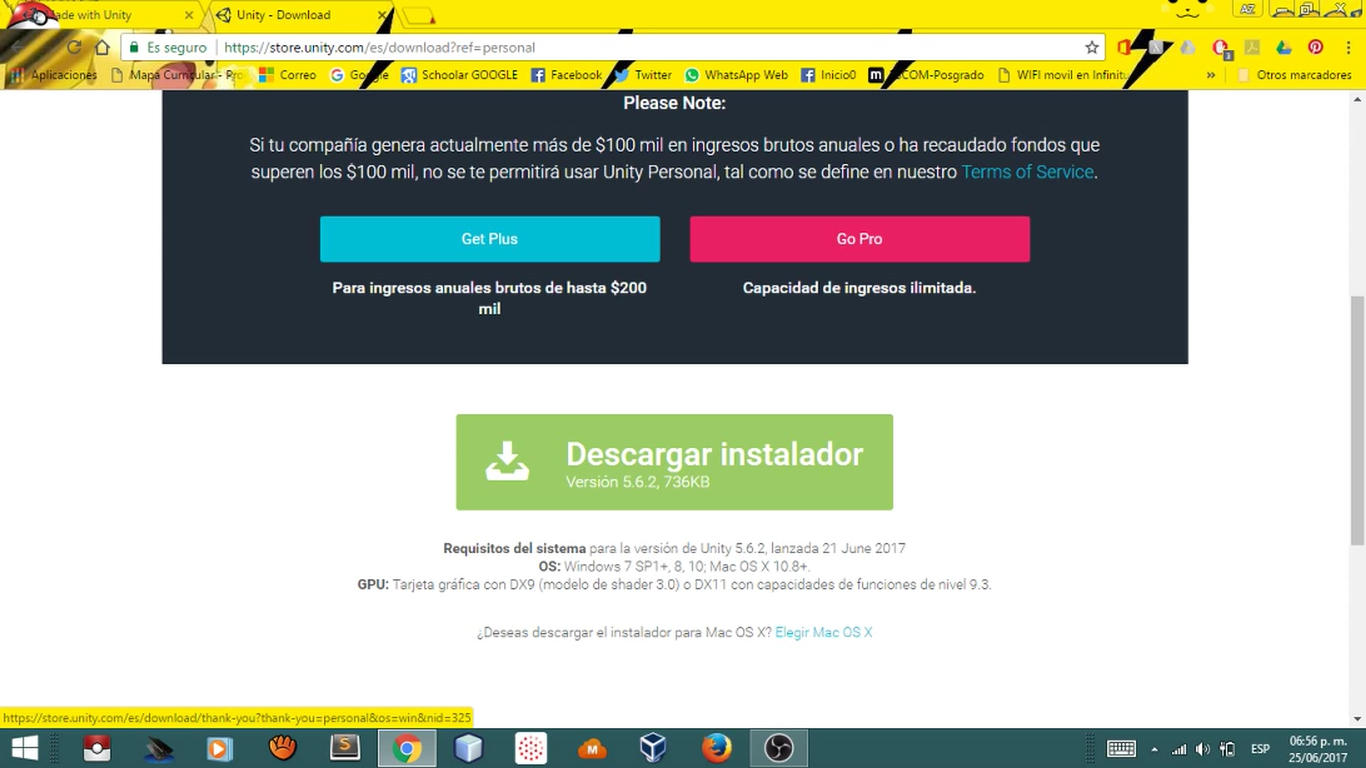
\includegraphics[width=\linewidth]{image/IU01}
  \end{itemize}
\end{frame}


\section{Instalaciones}

\subsection{Unity 5.6.2}

\begin{frame}{01}{Optional Subtitle}
  \begin{itemize}
  \item {
    Nos dirigimos a la página oficial de Unity:
    https://store.unity.com/es
  }
  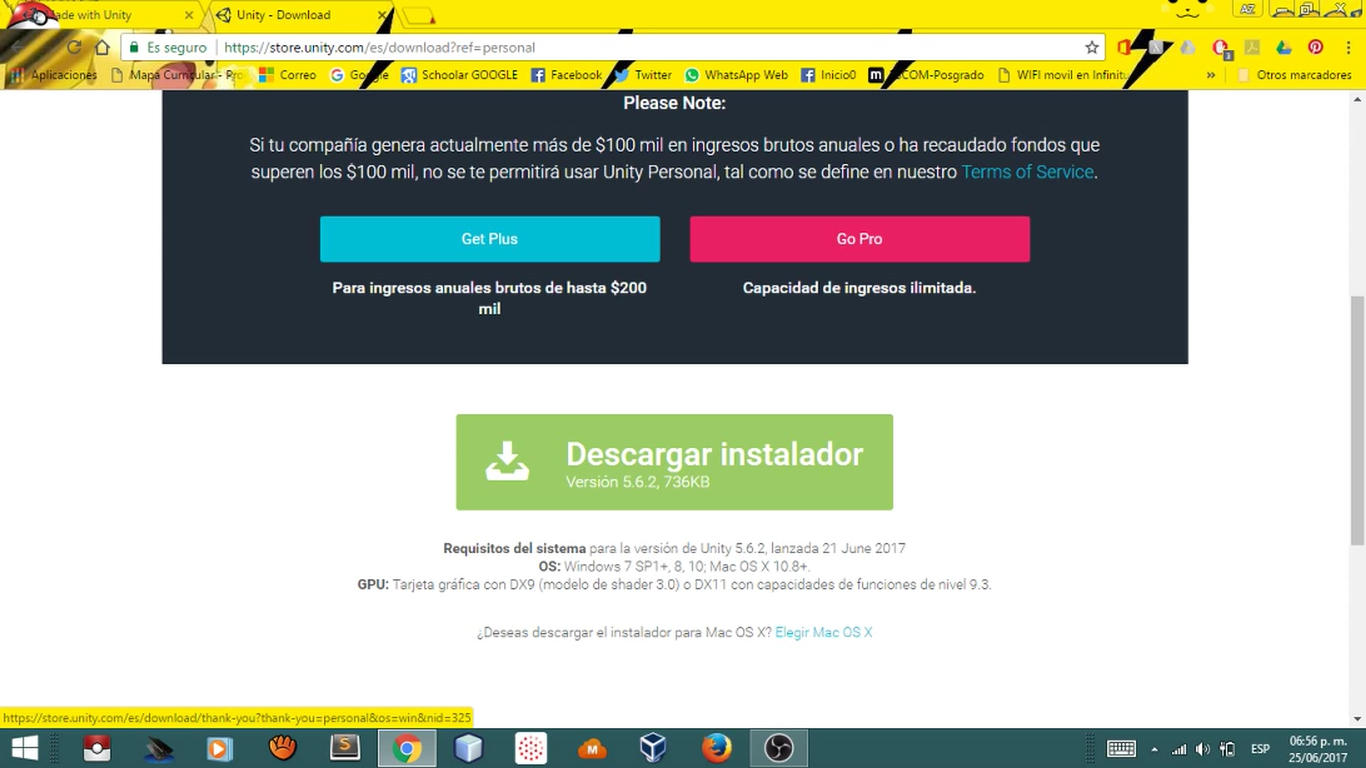
\includegraphics[width=\linewidth]{image/IU01}
  \item {
    En este caso utilizaremos la versión "Personal"
  }
  \end{itemize}
\end{frame}

%COPIA Y PEGA ESTE  PEDAZO PARA AGREGAR UNA DIAPOSITIVA
\begin{frame}{02}{Optional Subtitle}
  \begin{itemize}
  \item {
    Aceptamos los términos de condición
  }
  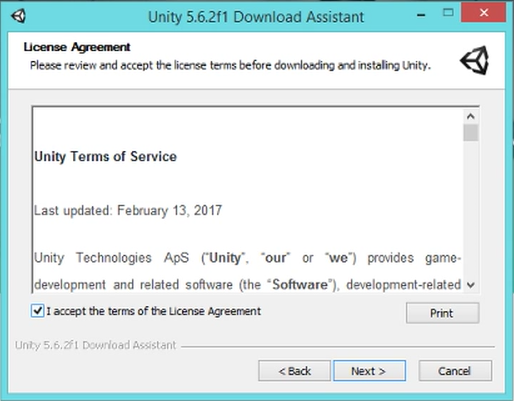
\includegraphics[width=\linewidth]{image/IU02}
  \end{itemize}
\end{frame}
%AQUI TERMINA EL PEDAZO A COPIAR Y PEGAR

\begin{frame}{03}{Optional Subtitle}
  \begin{itemize}
  \item {
    En los paquetes a instalar seleccionamos la opción de soporte para android
  }
  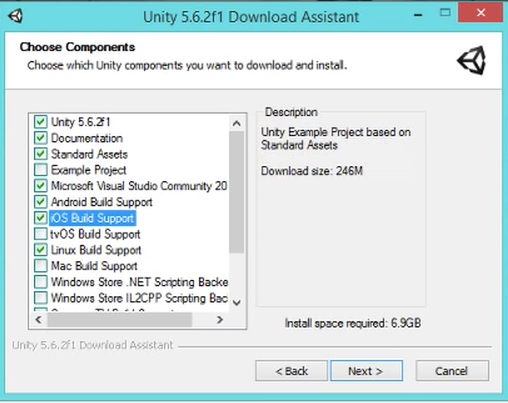
\includegraphics[width=\linewidth, height=0.7\paperheight]{image/IU03}
  \end{itemize}
\end{frame}

\begin{frame}{04}{Optional Subtitle}
  \begin{itemize}
  \item {
    Al terminar de instalar va a pedir acceder a las redes
  }
  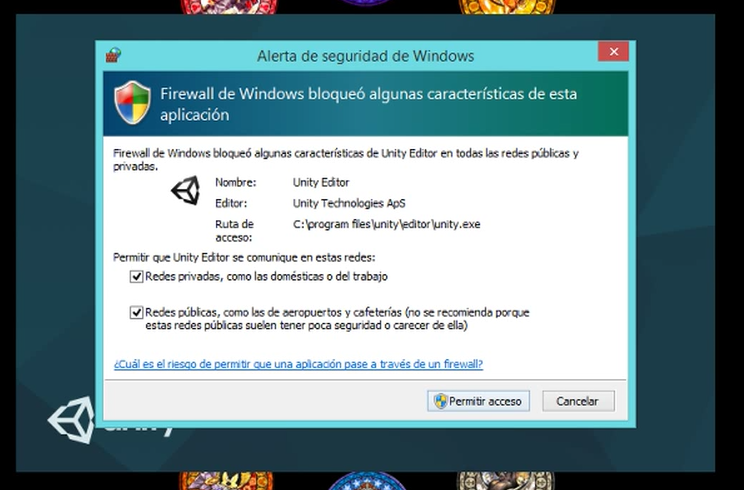
\includegraphics[width=\linewidth]{image/IU04}

  \end{itemize}
\end{frame}

\begin{frame}{05}{Optional Subtitle}
  \begin{itemize}
  \item {
    Nos va apedir una cuenta Unity para poder usarlo
  }
  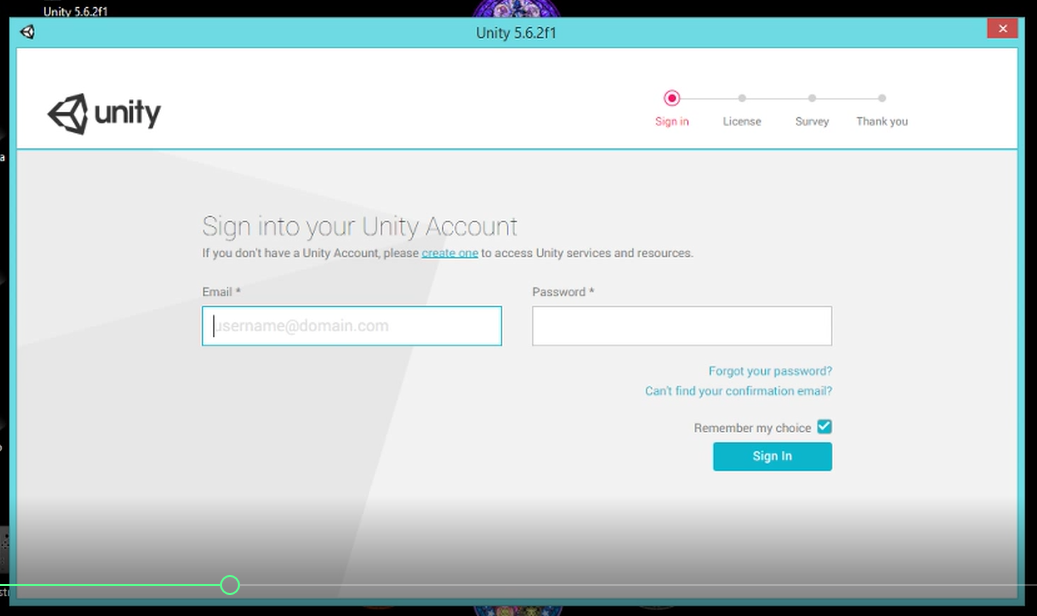
\includegraphics[width=\linewidth]{image/IU05}

  \end{itemize}
\end{frame}

\begin{frame}{06}{Optional Subtitle}
  \begin{itemize}
  \item {
    Creamos una cuenta
  }
  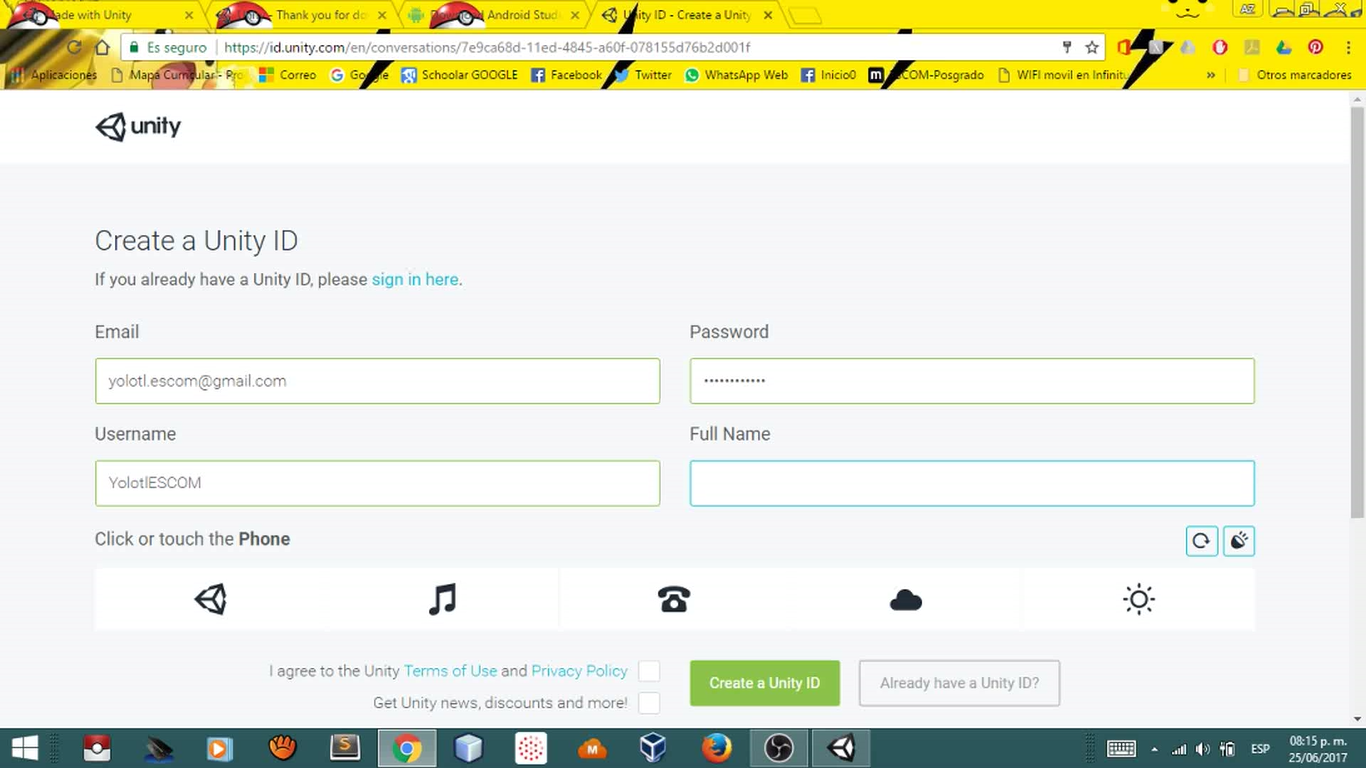
\includegraphics[width=\linewidth]{image/IU06}

  \end{itemize}
\end{frame}

\begin{frame}{07}{Optional Subtitle}
  \begin{itemize}
  \item {
    Nos mandará un correo electrónico para confirmación de datos
  }
  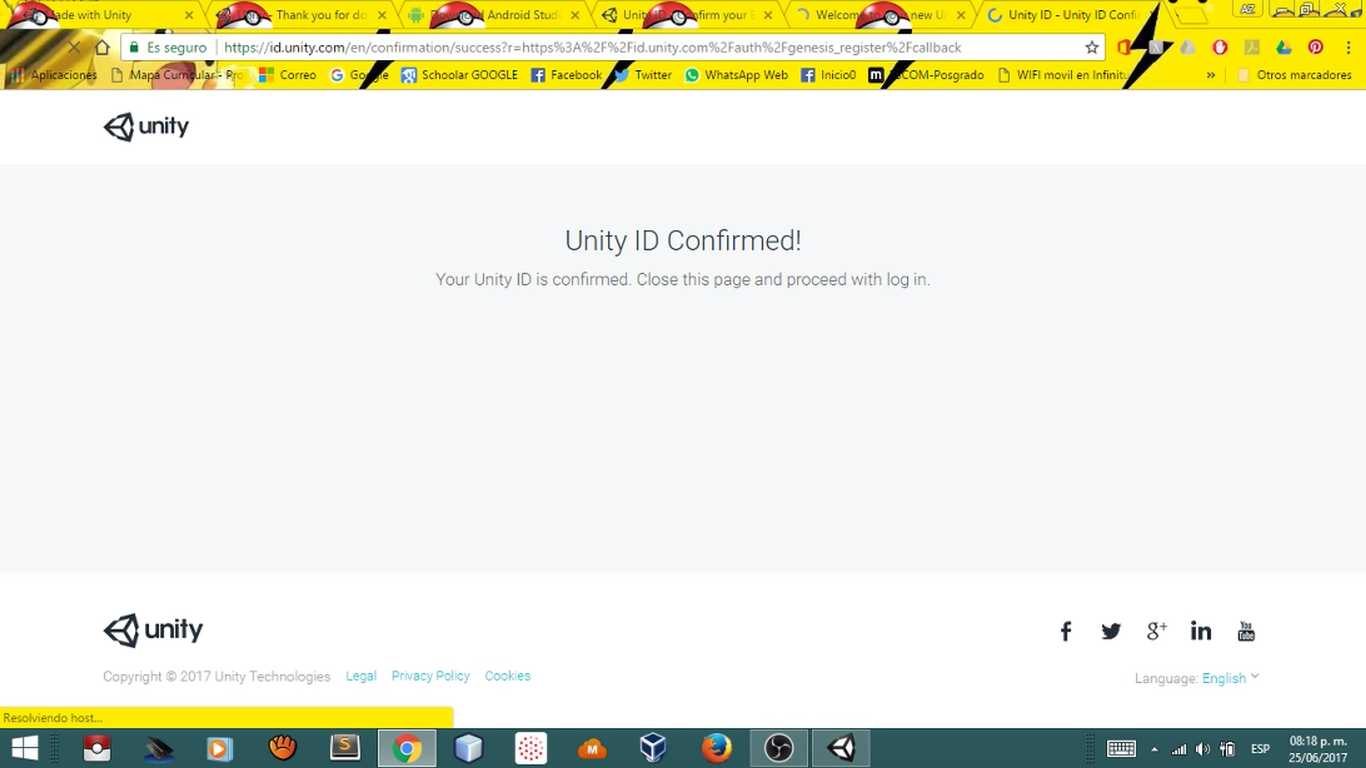
\includegraphics[width=\linewidth]{image/IU07}

  \end{itemize}
\end{frame}

\begin{frame}{08}{Optional Subtitle}
  \begin{itemize}
  \item {
    Ahora si podemos ingresar
  }
  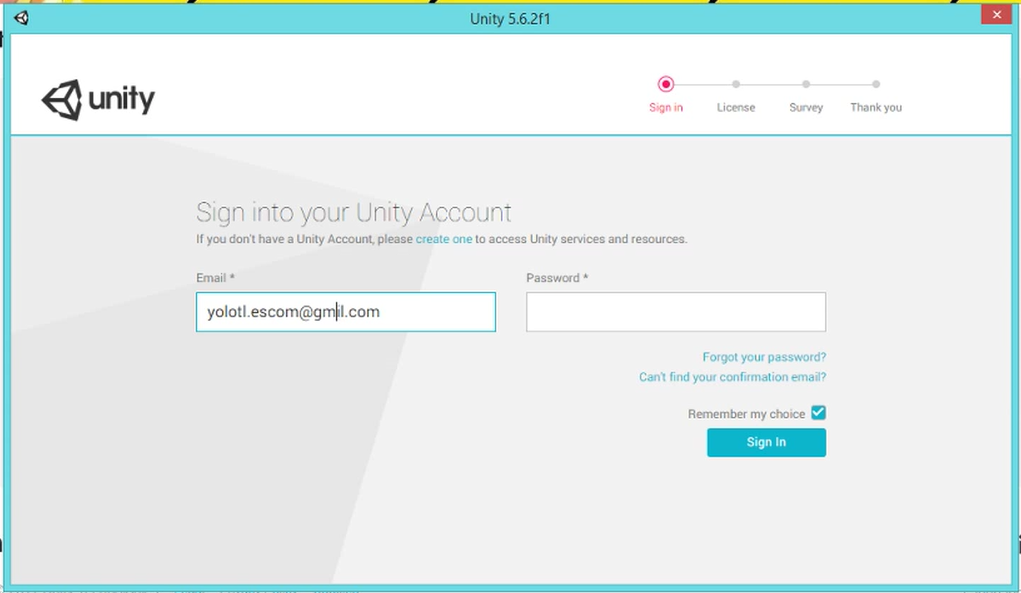
\includegraphics[width=\linewidth]{image/IU08}

  \end{itemize}
\end{frame}

\begin{frame}{09}{Optional Subtitle}
  \begin{itemize}
  \item {
    Opcionalmente llenamos un cuestionario
  }
  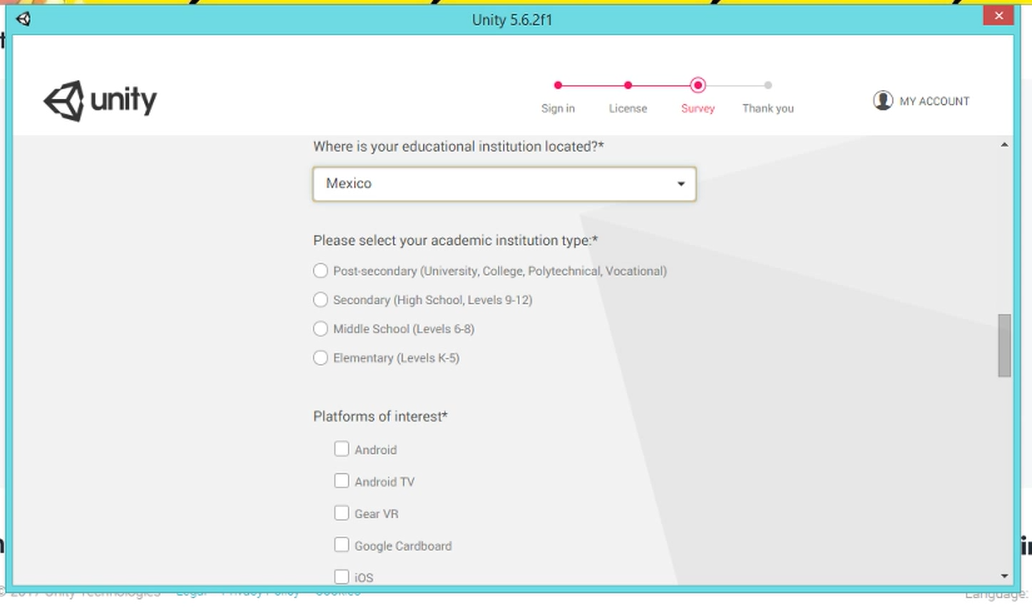
\includegraphics[width=\linewidth]{image/IU09}
  \end{itemize}
\end{frame}

\begin{frame}{10}{Optional Subtitle}
  \begin{itemize}
  \item {
    Y se abre ya la aplicación de Unity
  }
  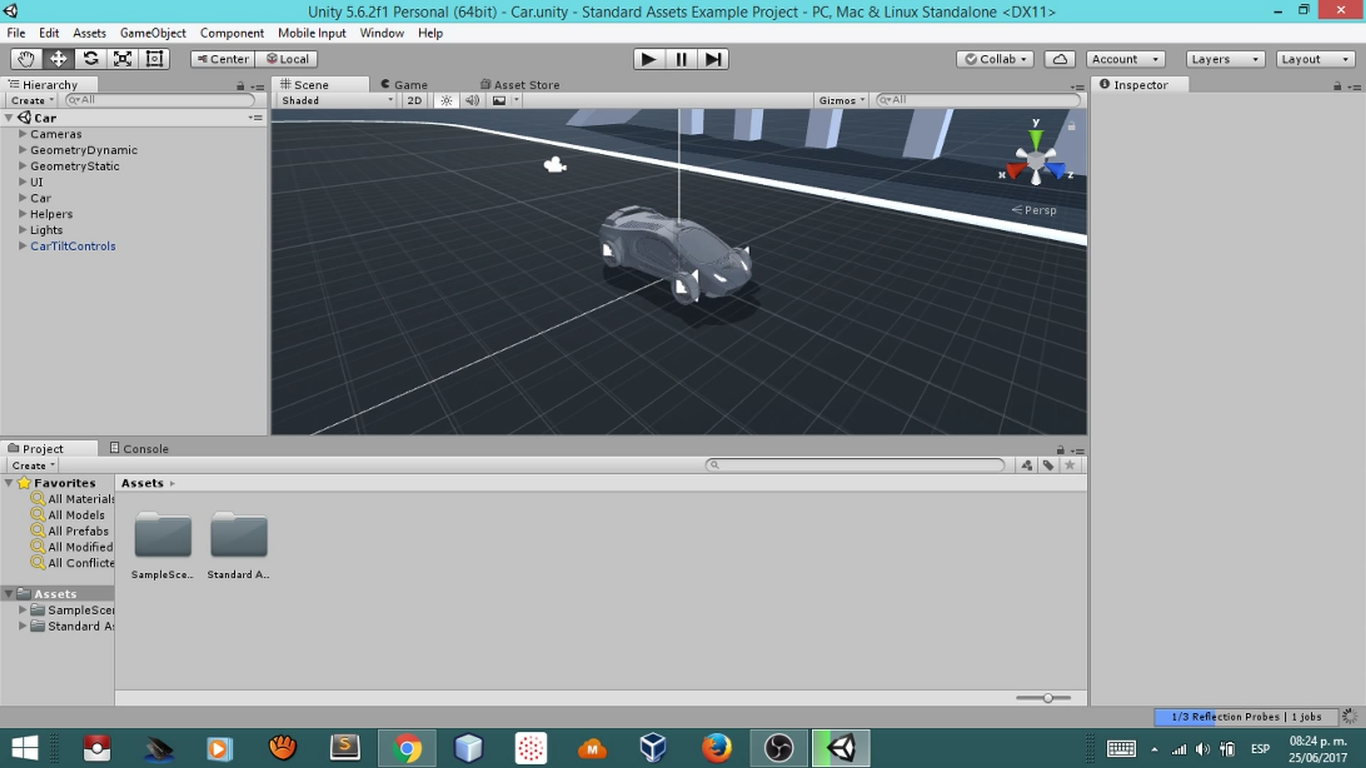
\includegraphics[width=\linewidth]{image/IU10}
  \end{itemize}
\end{frame}

\subsection{Android Studio 2.3.3}

\begin{frame}{11}{Optional Subtitle}
  \begin{itemize}
  \item {
    Vamos a la página oficial de Android Studio para descargar el instalador
  }
  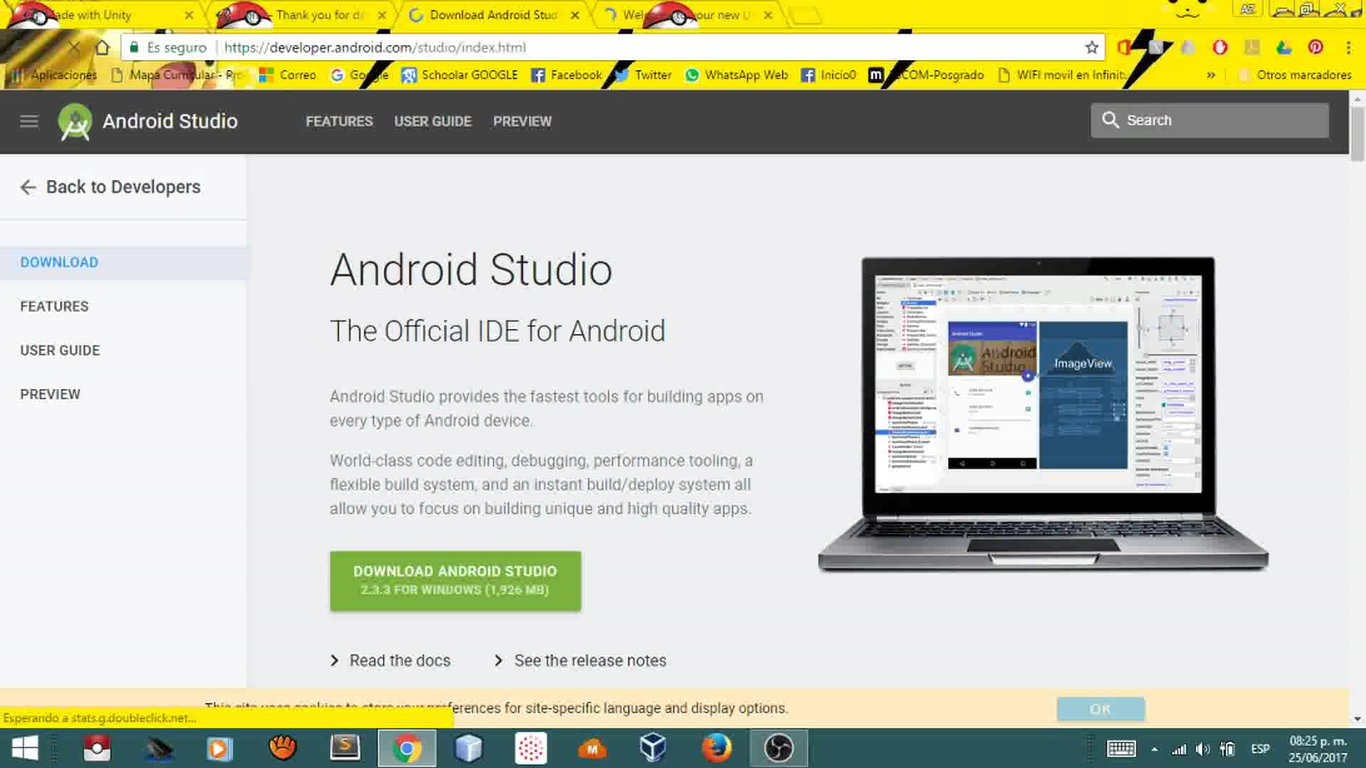
\includegraphics[width=\linewidth]{image/IU11}
  \end{itemize}
\end{frame}

\begin{frame}{12}{Optional Subtitle}
  \begin{itemize}
  \item {
    Ejecutamos el instalador
  }
  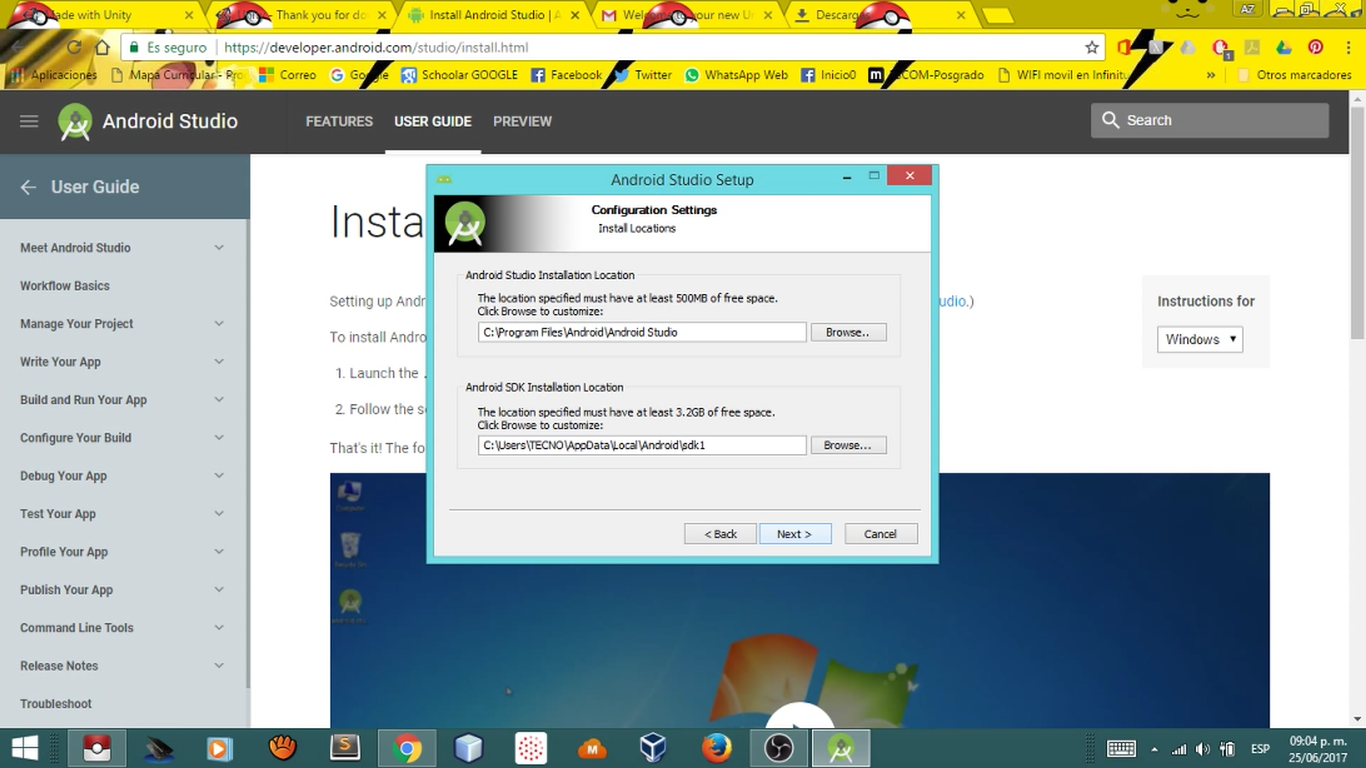
\includegraphics[width=\linewidth]{image/IU12}
  \end{itemize}
\end{frame}

\begin{frame}{13}{Optional Subtitle}
  \begin{itemize}
  \item {
    Se abrirá Android Studio para verificar paquetes y seguir instalando y actualizando
  }
  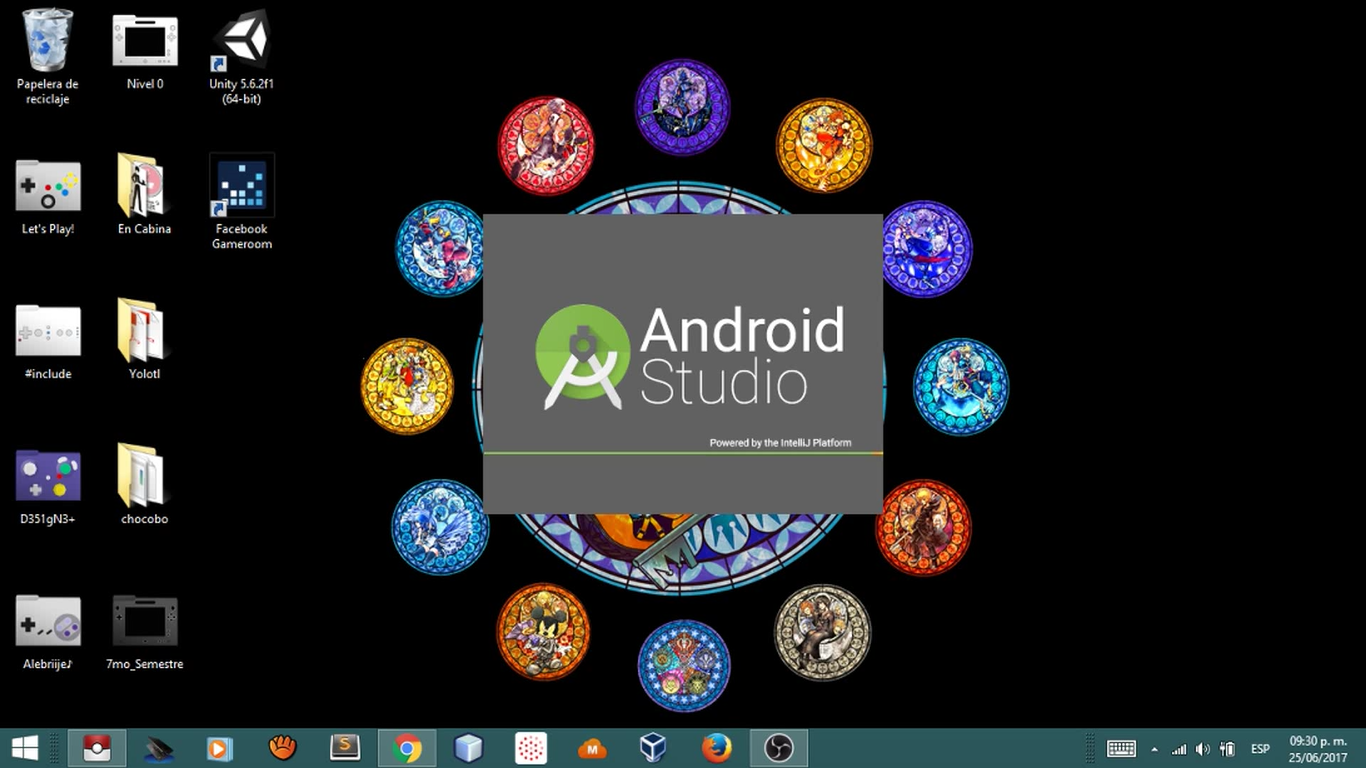
\includegraphics[width=\linewidth]{image/IU13}
  \end{itemize}
\end{frame}

\begin{frame}{14}{Optional Subtitle}
  \begin{itemize}
  \item {
   Abrimos Android Studio
  }
  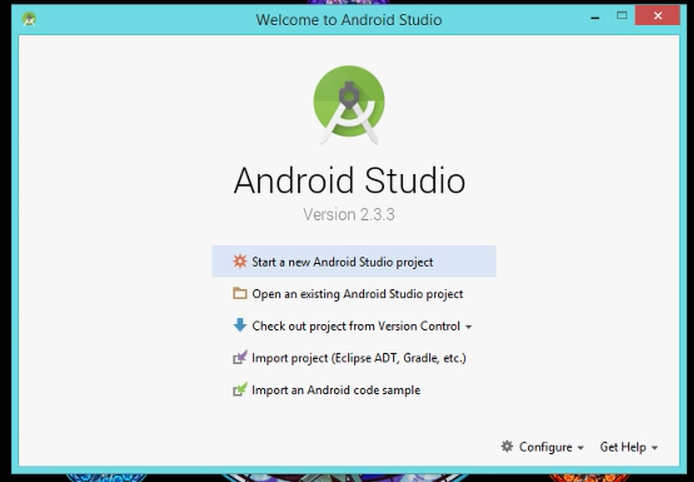
\includegraphics[width=\linewidth]{image/IU14}
  \end{itemize}
\end{frame}

\begin{frame}{15}{Optional Subtitle}
  \begin{itemize}
  \item {
    Le damos permisos de uso de redes
  }
  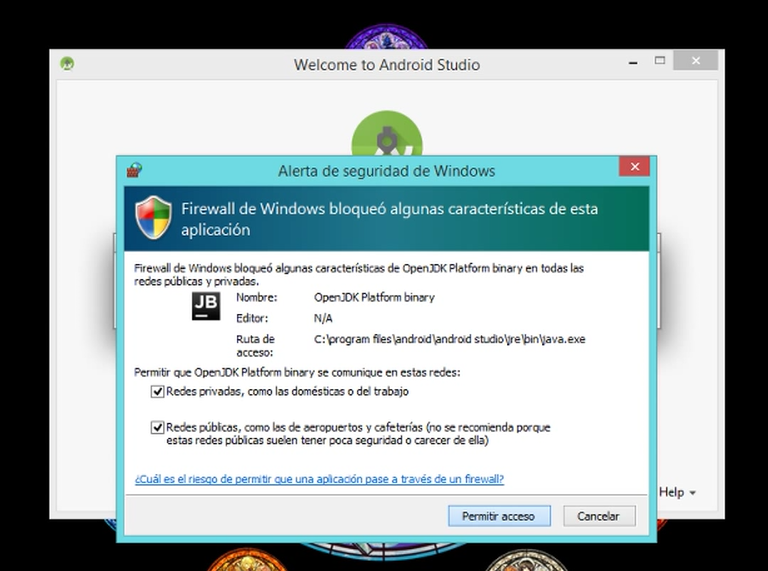
\includegraphics[width=\linewidth]{image/IU15}
  \end{itemize}
\end{frame}

\begin{frame}{16}{Optional Subtitle}
  \begin{itemize}
  \item {
    Nos vamos a “SDK Manager”
  }
  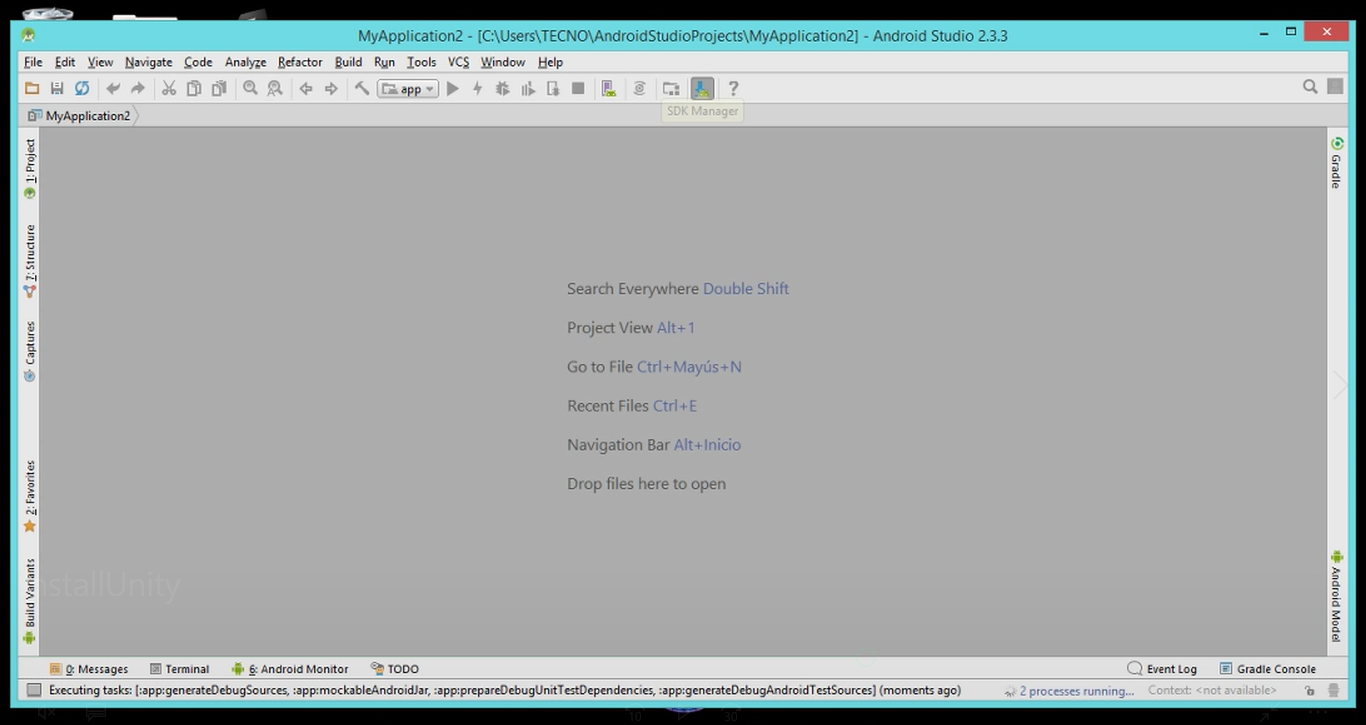
\includegraphics[width=\linewidth]{image/IU16}
  \end{itemize}
\end{frame}

\begin{frame}{17}{Optional Subtitle}
  \begin{itemize}
  \item {
   Descargamos las versiones de Android que vayamos a autilizar para nuestro proyecto en “SDK Platforms”
  }
  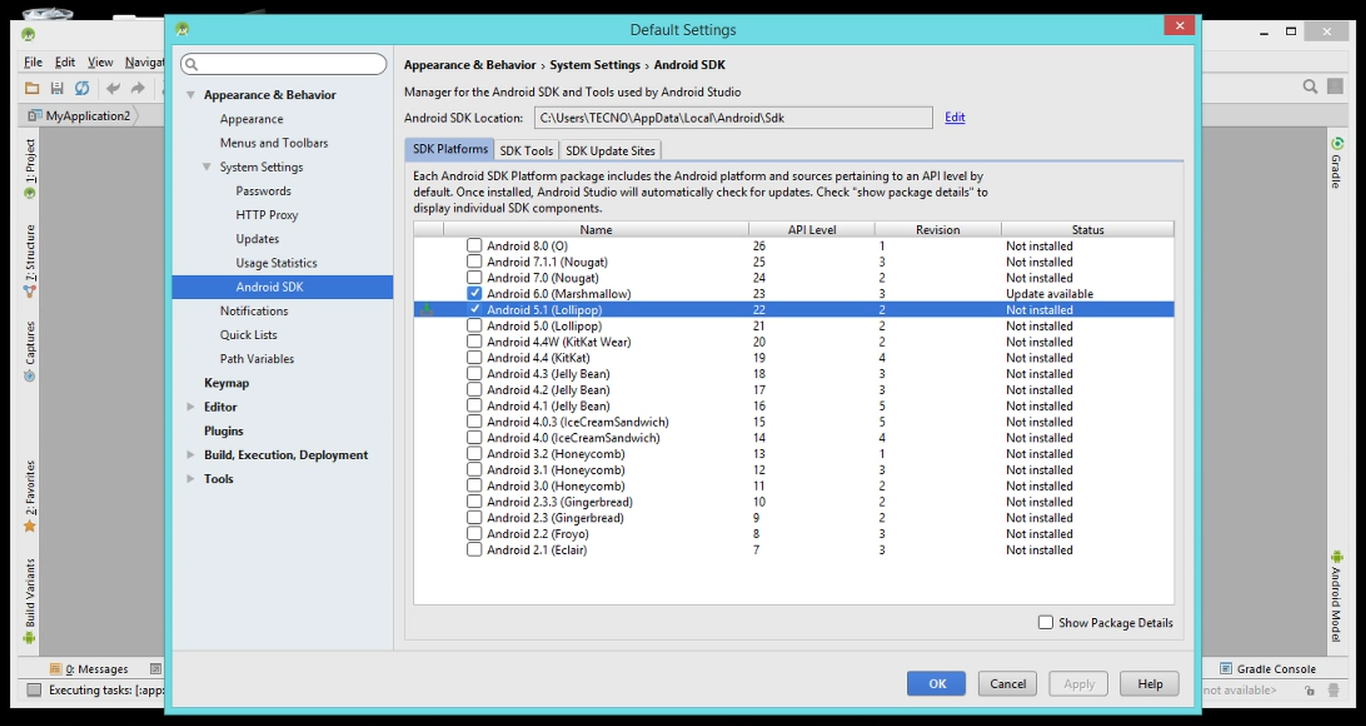
\includegraphics[width=\linewidth]{image/IU17}
  \end{itemize}
\end{frame}

\begin{frame}{18}{Optional Subtitle}
  \begin{itemize}
  \item {
    En “SDK Tools” nos aseguramos que tengamos los paquetes:
•	Android support repository
•	Google play APK Expansion Library
•	Android SDK Build-Tools
•	Android SDK Tools
•	Android SDK Platforms-Tools

  }
  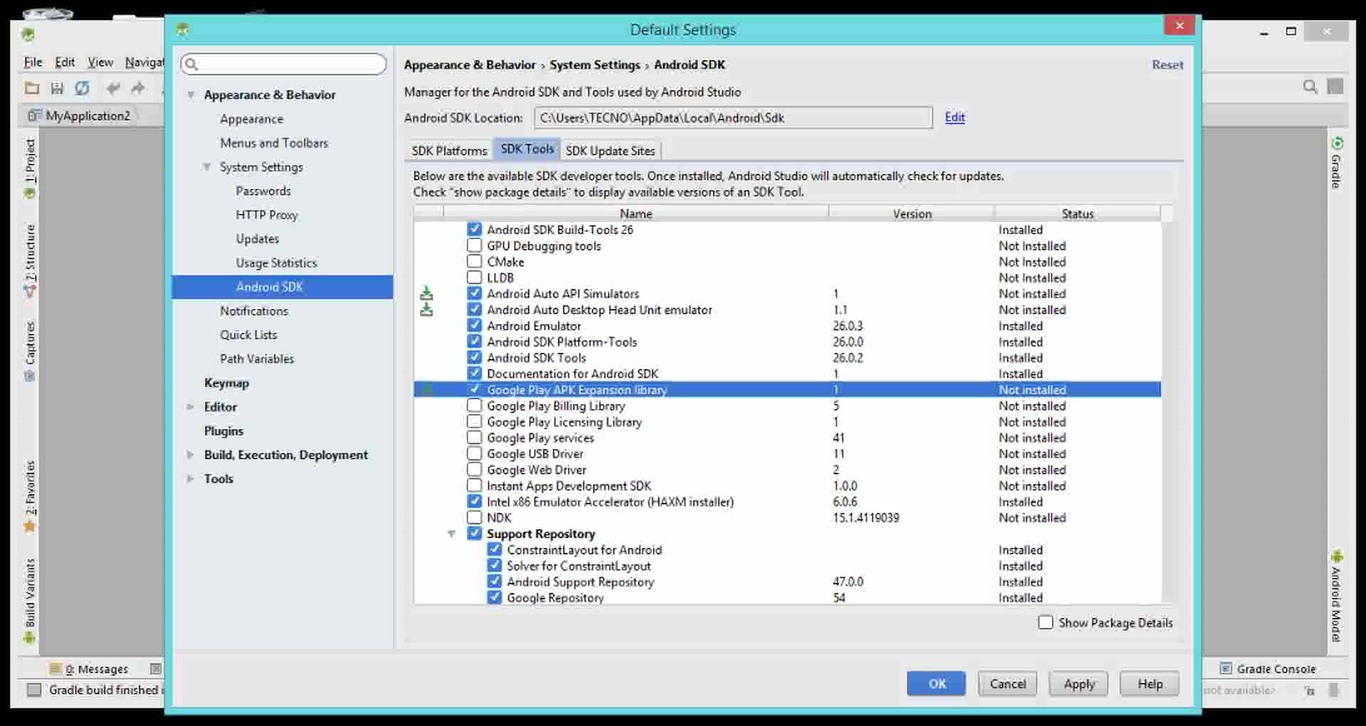
\includegraphics[width=\linewidth]{image/IU18}
  \end{itemize}
\end{frame}

\begin{frame}{19}{Optional Subtitle}
  \begin{itemize}
  \item {
    Unity necesita una versión específica de la carpeta “tools” dentro del SDK de Android Studio, la 25.2.5
La hemos descargado de una liga de un foro
  }
  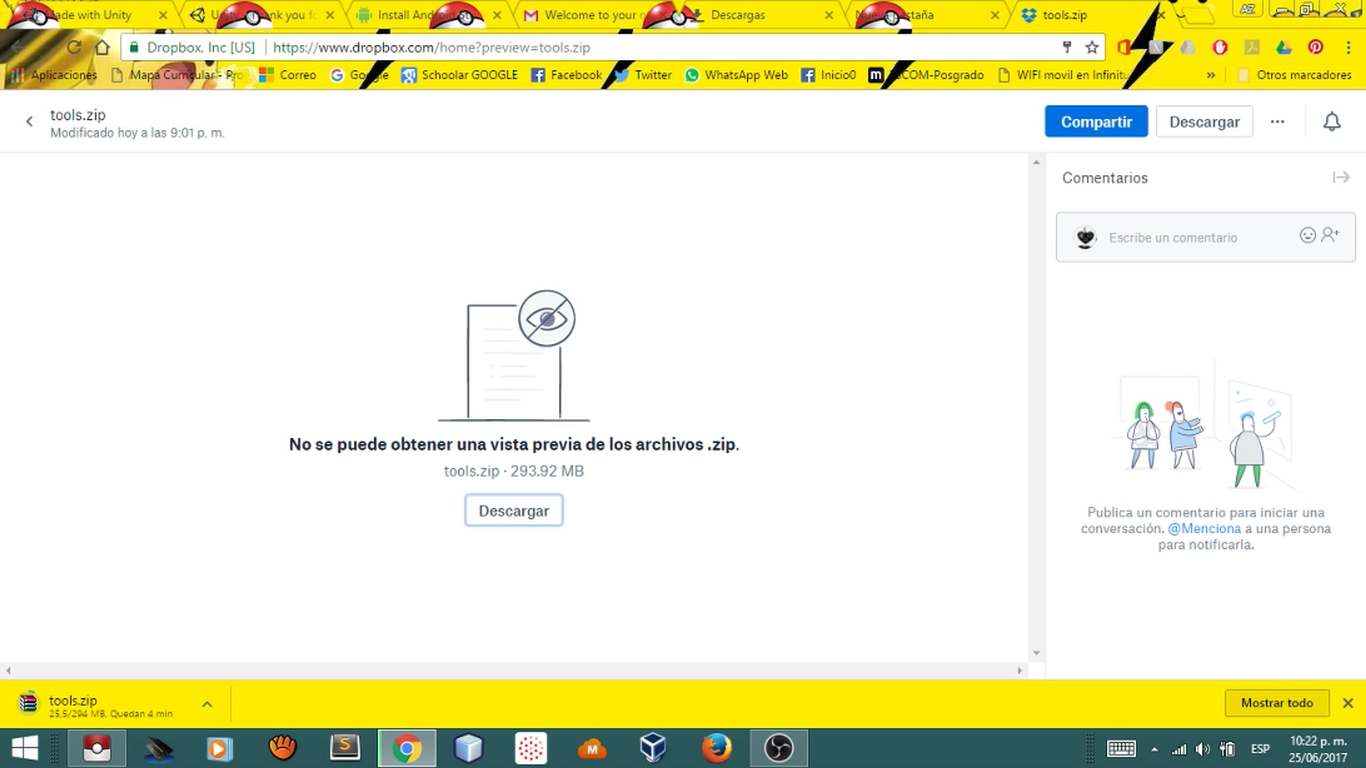
\includegraphics[width=\linewidth]{image/IU19}
  \end{itemize}
\end{frame}

\begin{frame}{20}{Optional Subtitle}
  \begin{itemize}
  \item {
   Y la sustituimos por la carpeta actual “tools” que se encuentra en:
	Equipo-Windows8_OS(C:)-Usuarios-TECNO(nombre del usuario o cuenta)-AppData(carpeta oculta)-Local-Android-SDK
  }
  
  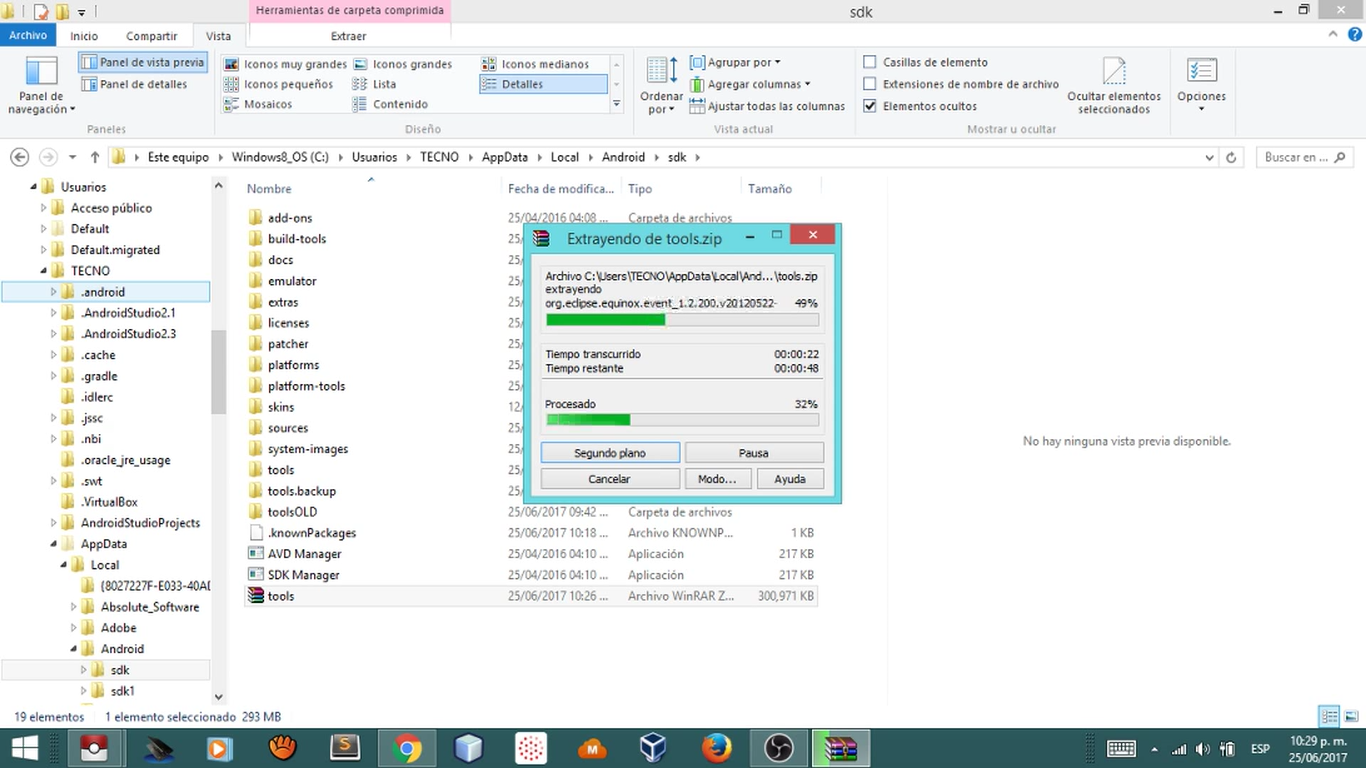
\includegraphics[width=\linewidth]{image/IU20}
  \end{itemize}
\end{frame}

\subsection{JDK 7 JAVA ORACLE}

\begin{frame}{21}{Optional Subtitle}
  \begin{itemize}
  \item {
    Unity solo tiene aceptada hasta la versión 7 del JDK
  }
  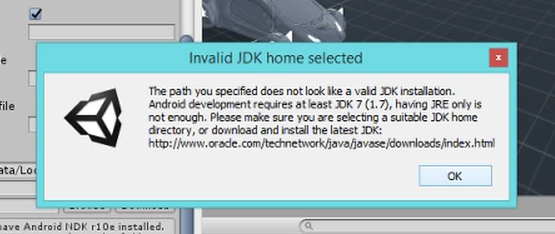
\includegraphics[width=\linewidth]{image/IU21}
  \end{itemize}
\end{frame}

\begin{frame}{22}{Optional Subtitle}
  \begin{itemize}
  \item {
    Nos vamos a l repositorio oficial de Oracle
  }
  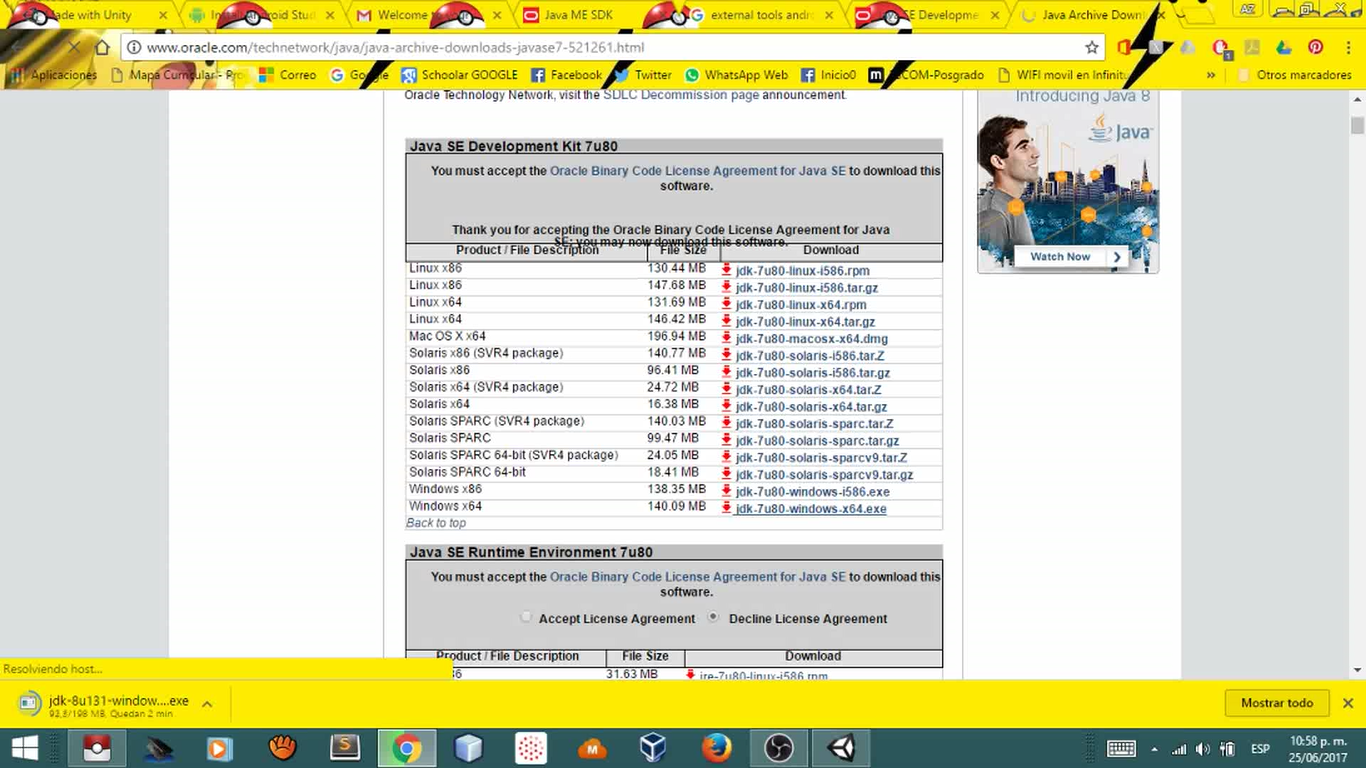
\includegraphics[width=\linewidth]{image/IU22}
  \end{itemize}
\end{frame}

\begin{frame}{23}{Optional Subtitle}
  \begin{itemize}
  \item {
    Para ello necesitamos una cuenta de Oracle, ya sea que ingresemos o podemos crearla.
  }
  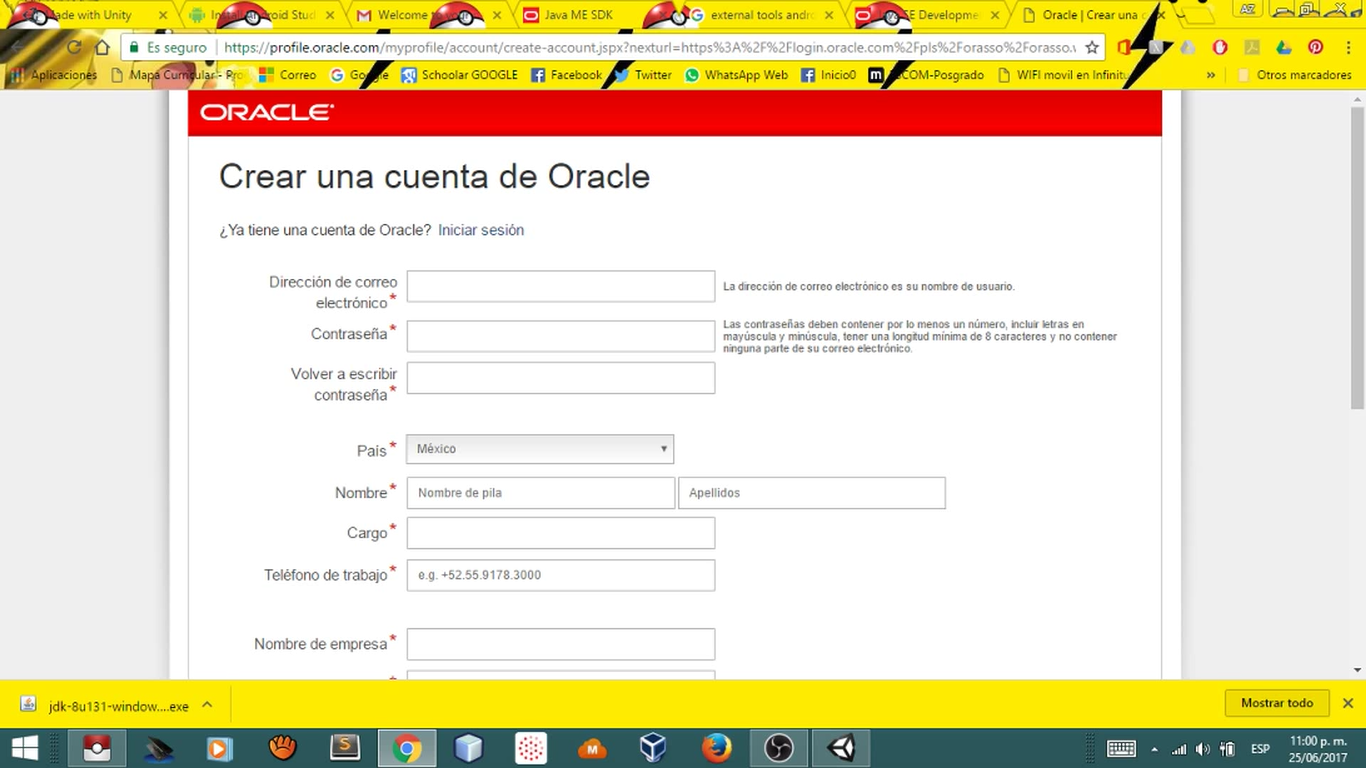
\includegraphics[width=\linewidth]{image/IU23}
  \end{itemize}
\end{frame}

\begin{frame}{24}{Optional Subtitle}
  \begin{itemize}
  \item {
    Verificamos con nuestro correo que ha llegado de confirmación
  }
  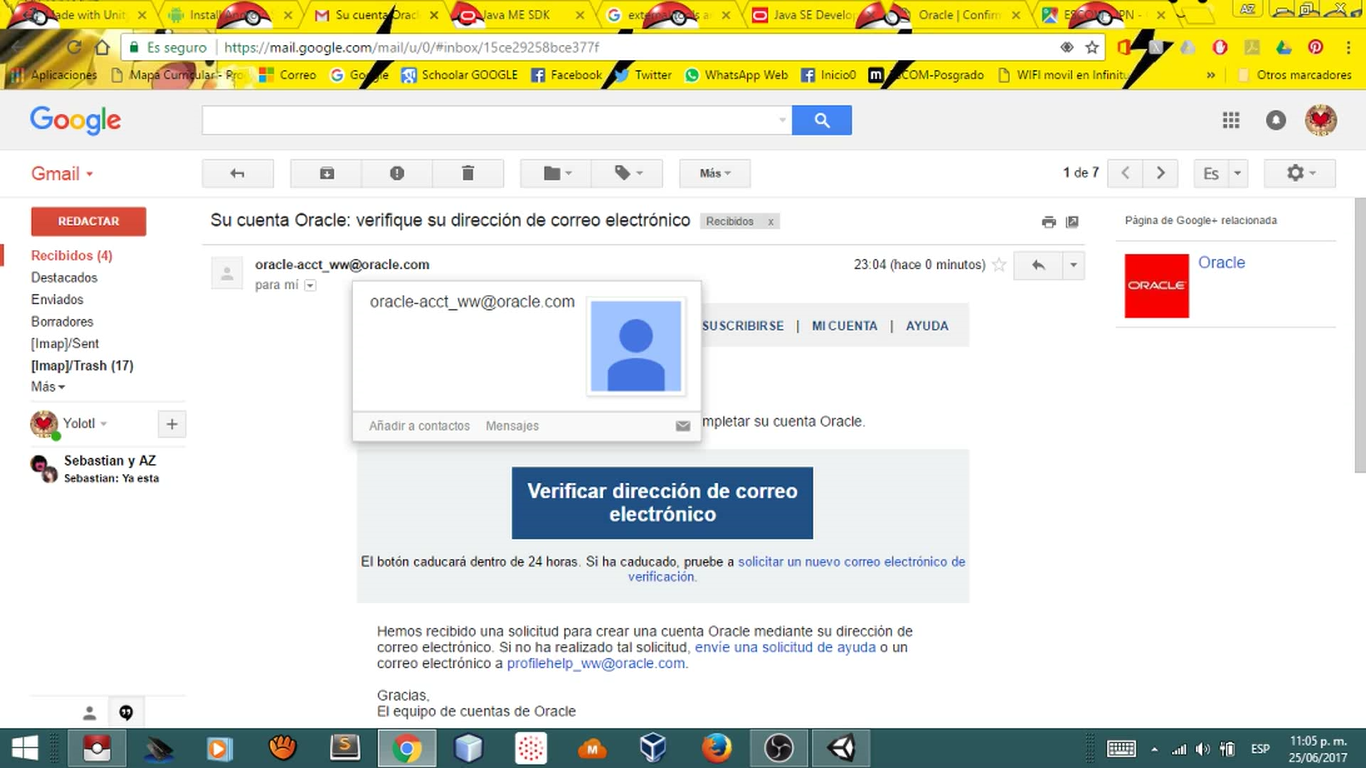
\includegraphics[width=\linewidth]{image/IU24}
  \end{itemize}
\end{frame}

\begin{frame}{25}{Optional Subtitle}
  \begin{itemize}
  \item {
    Y ejecutamos el instalador
  }
  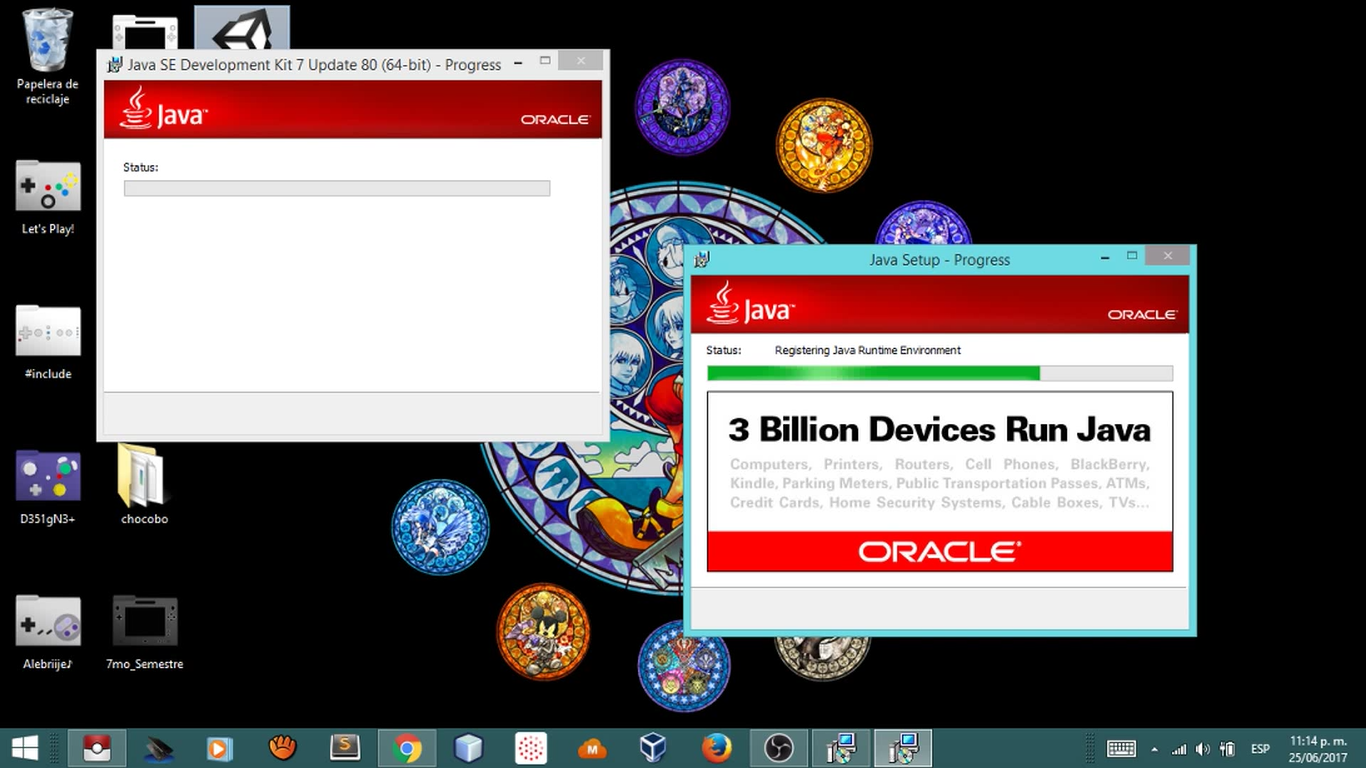
\includegraphics[width=\linewidth]{image/IU25}
  \end{itemize}
\end{frame}

%%ESTE PEDAZO PUEDE SERVIR
% You can reveal the parts of a slide one at a time
% with the \pause command:
%\begin{frame}{Second Slide Title}
%  \begin{itemize}
%  \item {
%    First item.
%    \pause % The slide will pause after showing the first item
%  }
%  \item {   
%    Second item.
%  }
  % You can also specify when the content should appear
  % by using <n->:
%  \item<3-> {
%    Third item.
%  }
%  \item<4-> {
%    Fourth item.
%  }
  % or you can use the \uncover command to reveal general
  % content (not just \items):
%  \item<5-> {
%    Fifth item. \uncover<6->{Extra text in the fifth item.}
%  }
%  \end{itemize}
%\end{frame}
%%FIN DE PEDAZO QUE PUEDE SERVIR

\section{Configuración}

\subsection{Android para Unity}

\begin{frame}{26}{Optional Subtitle}
  \begin{itemize}
  \item {
   Abrimos Unity y nos vamos a:
Edit –> Preferences… -> External Tools
  }
  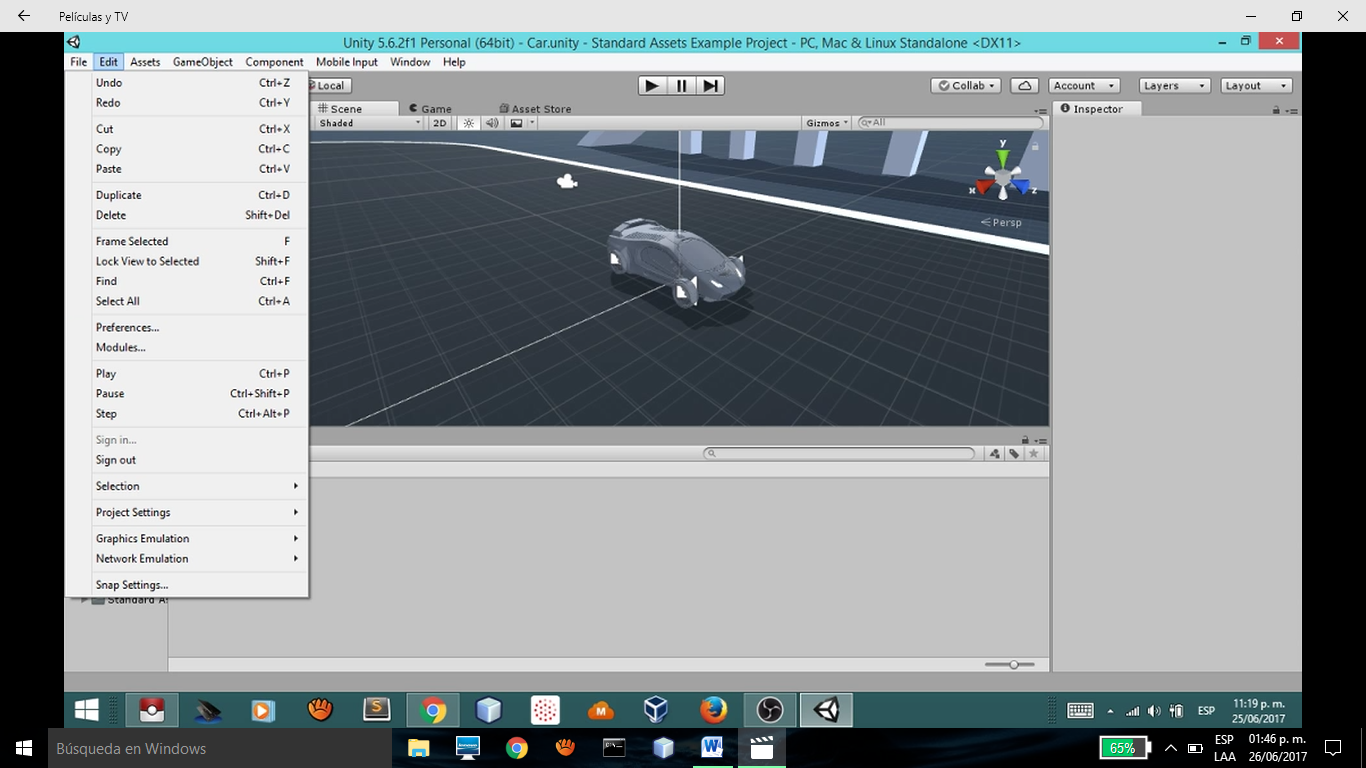
\includegraphics[width=\linewidth]{image/IU26}
  \end{itemize}
\end{frame}

\begin{frame}{27}{Optional Subtitle}
    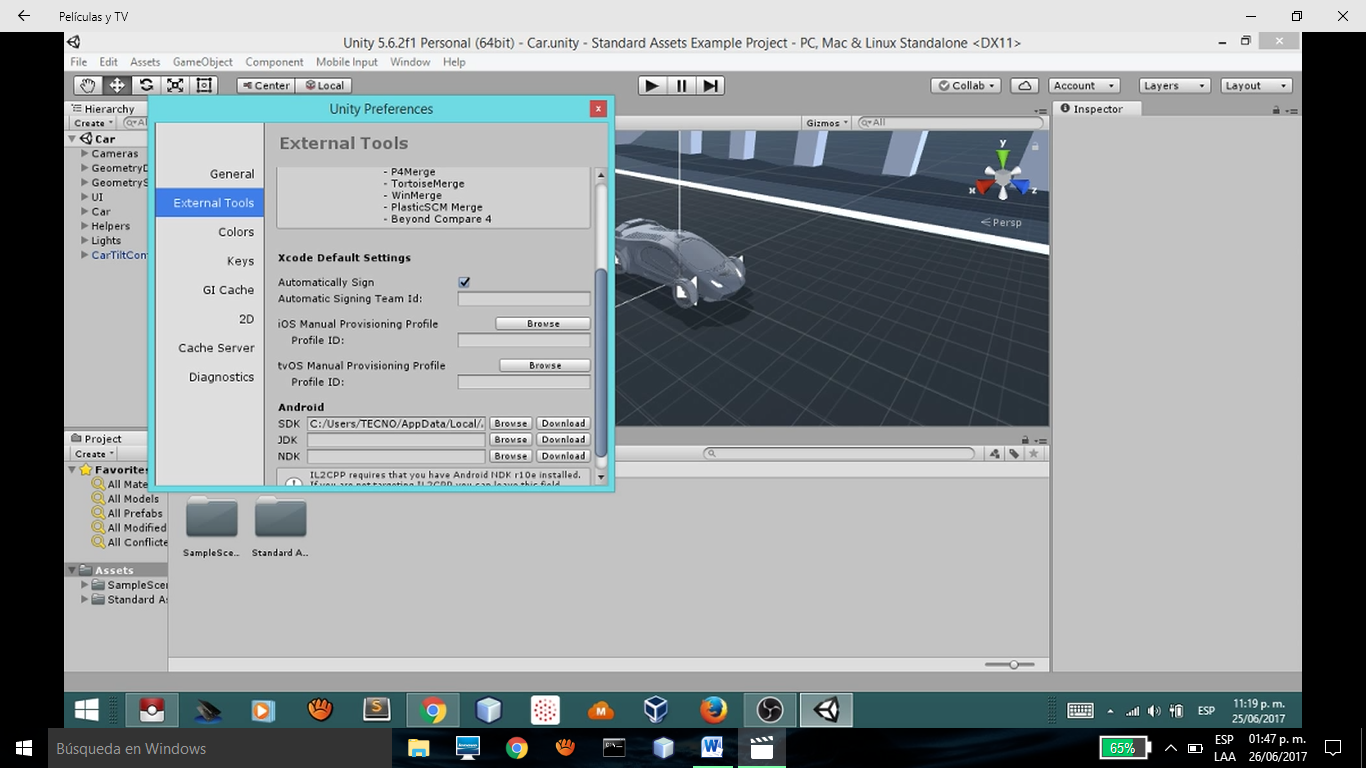
\includegraphics[width=\linewidth]{image/IU27}
\end{frame}

\begin{frame}{28}{Optional Subtitle}
  \begin{itemize}
  \item {
   En el apartado de android le damos las direcciones de donde se encuentran los SDK de Android Studios y JDK de Oracle
  }
  
  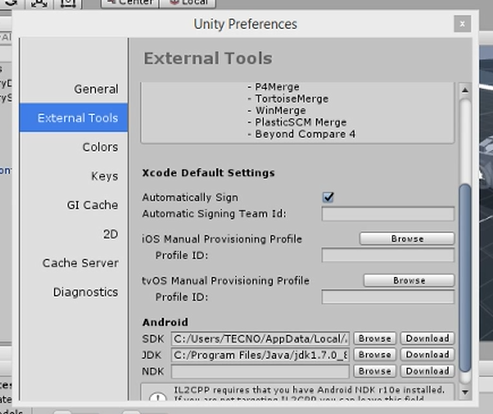
\includegraphics[width=\linewidth, height=0.6\paperheight]{image/IU28}
  \centering
  \end{itemize}
\end{frame}

\begin{frame}{29}{Optional Subtitle}
  \begin{itemize}
  \item {
    Abrimos nuestro proyecto a trabajar y nos vamos a:
File -> Build Settings… -> Player Settings -> Identification
Para asegurarnos de que se creará para la versión que queramos

  }
  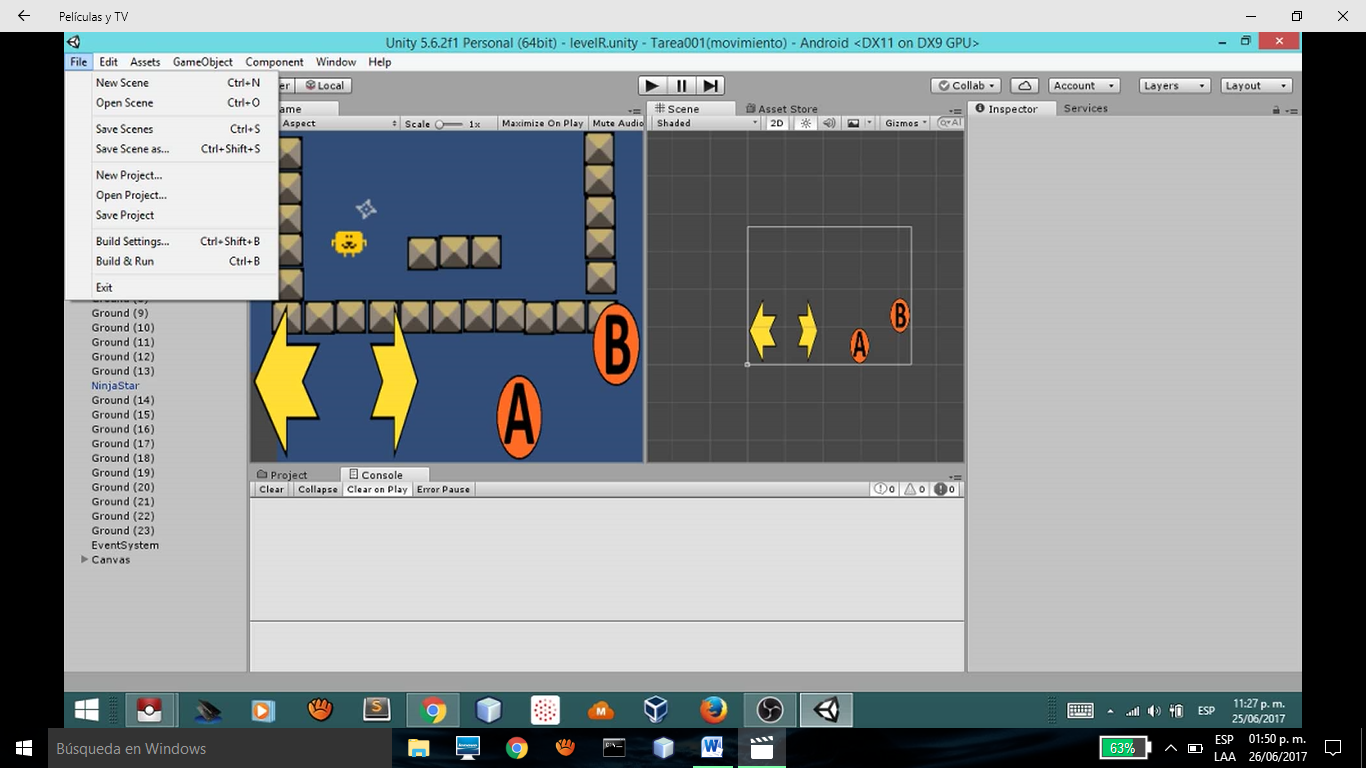
\includegraphics[width=\linewidth]{image/IU29}
  \end{itemize}
\end{frame}

\begin{frame}{30}{Optional Subtitle}
  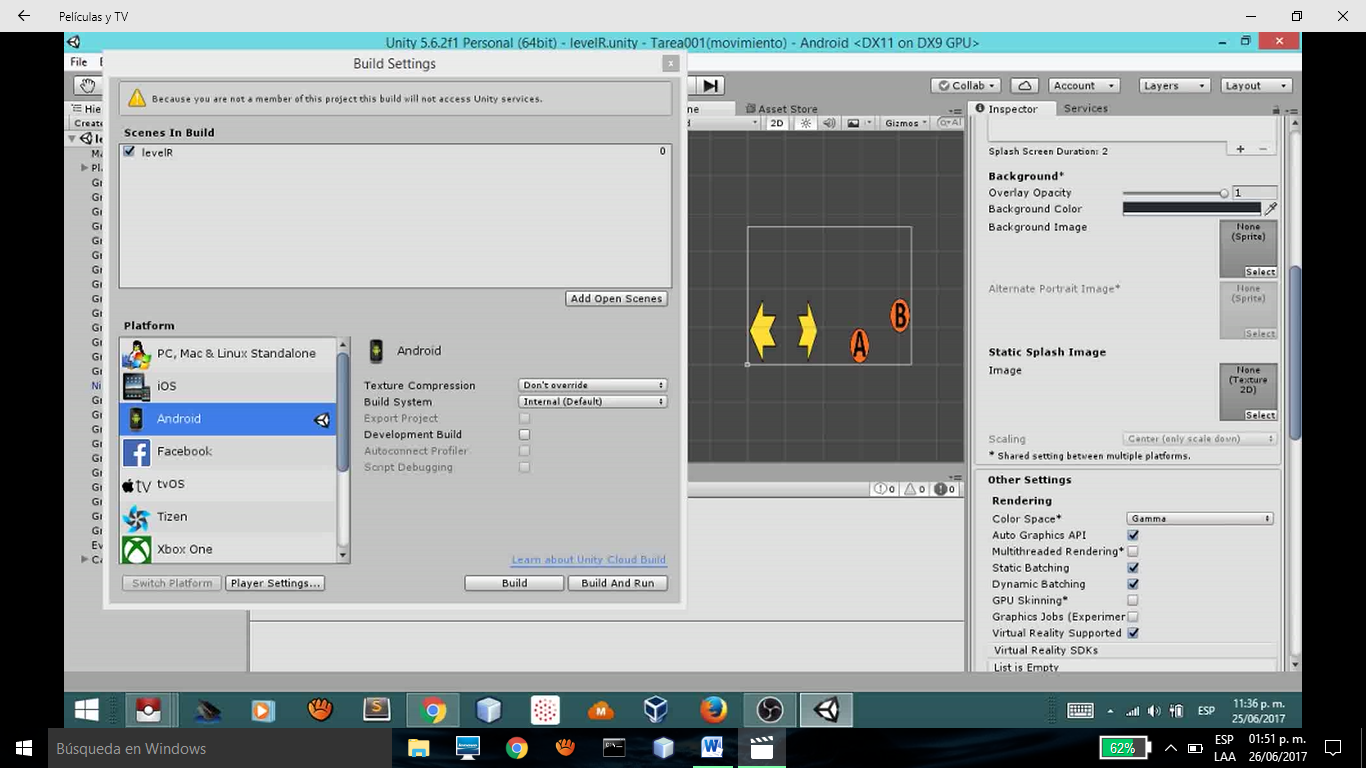
\includegraphics[width=\linewidth]{image/IU30}
\end{frame}

\begin{frame}{31}{Optional Subtitle}
  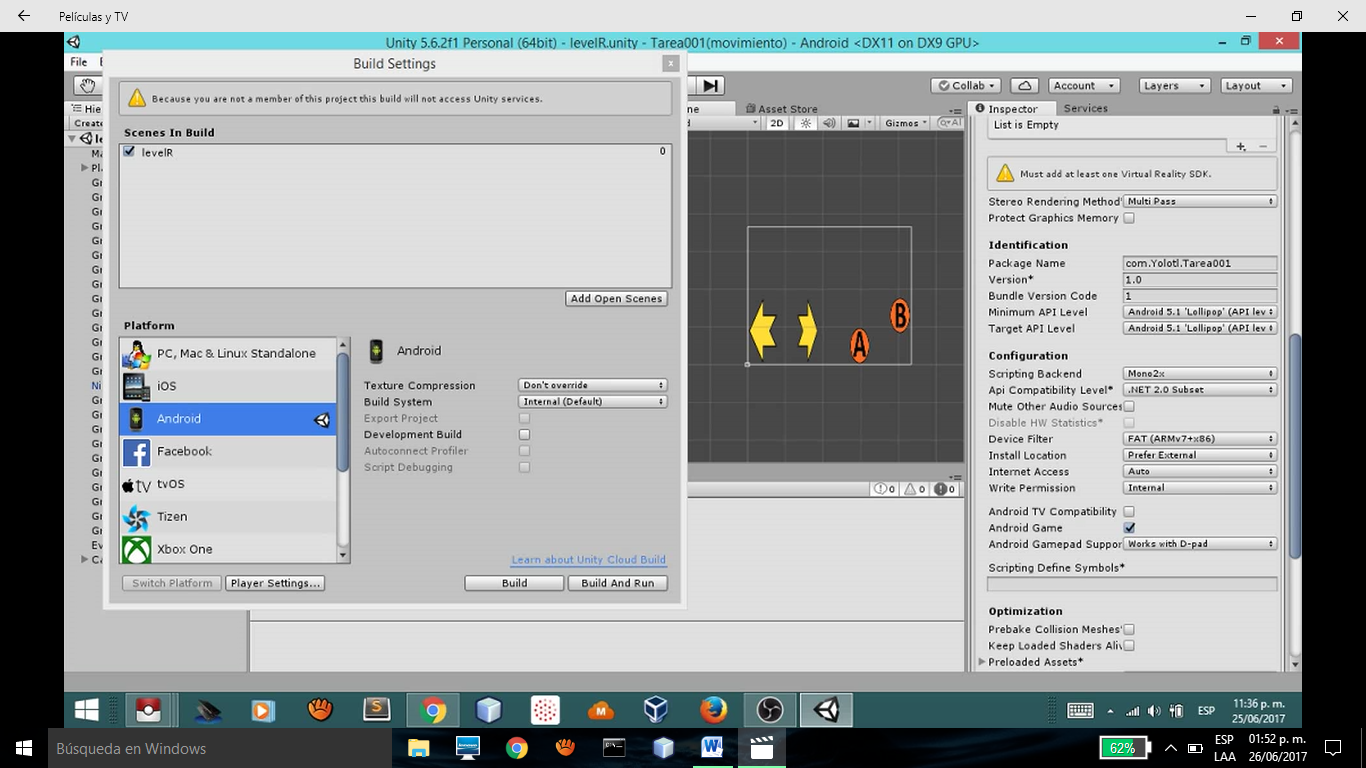
\includegraphics[width=\linewidth]{image/IU31}
\end{frame}

\begin{frame}{32}{Optional Subtitle}
  \begin{itemize}
  \item {
    Y oprimimos “Build” para crear el APK
  }
  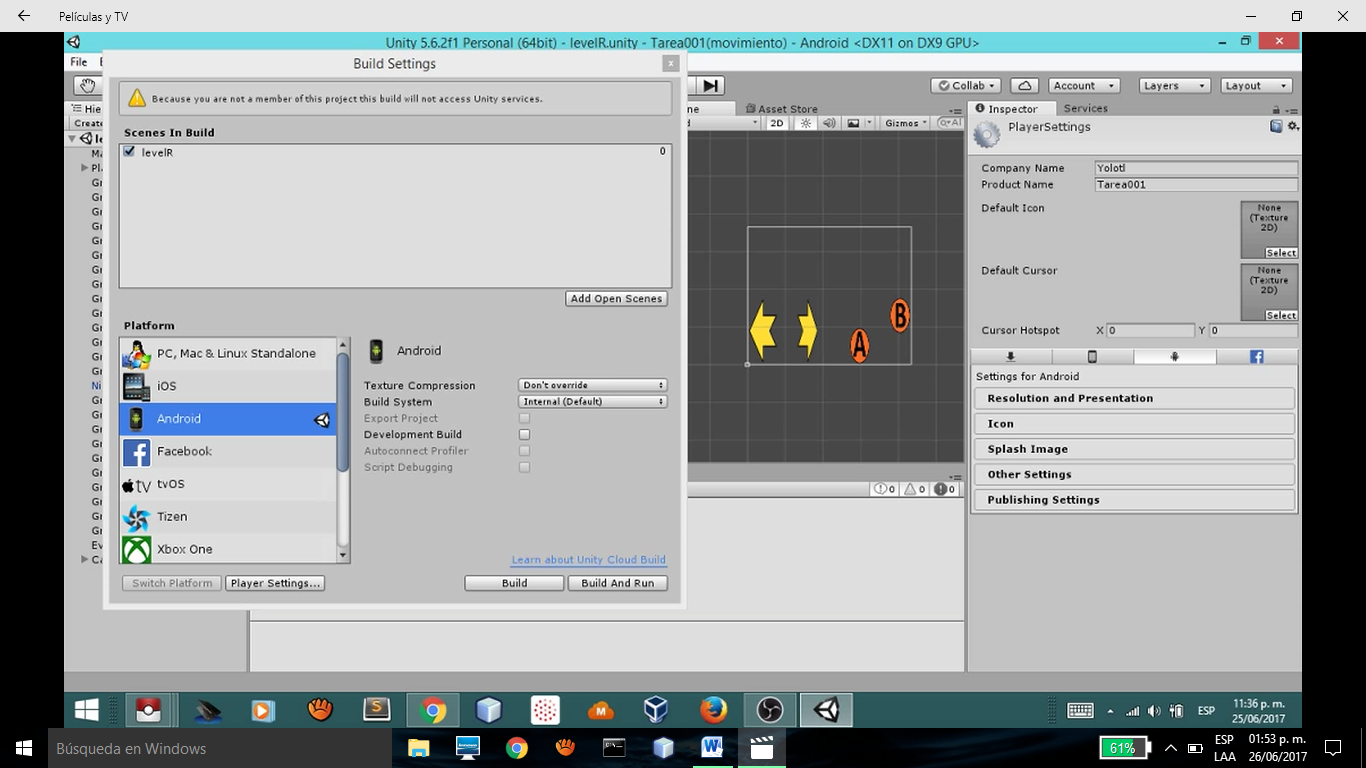
\includegraphics[width=\linewidth]{image/IU32}
  \end{itemize}
\end{frame}

\subsection{Dispositivo Android 5.1}

\begin{frame}{33}{Optional Subtitle}
  \begin{itemize}
  \item {
    Copiamos nuestro APK al dispositivo
  }
  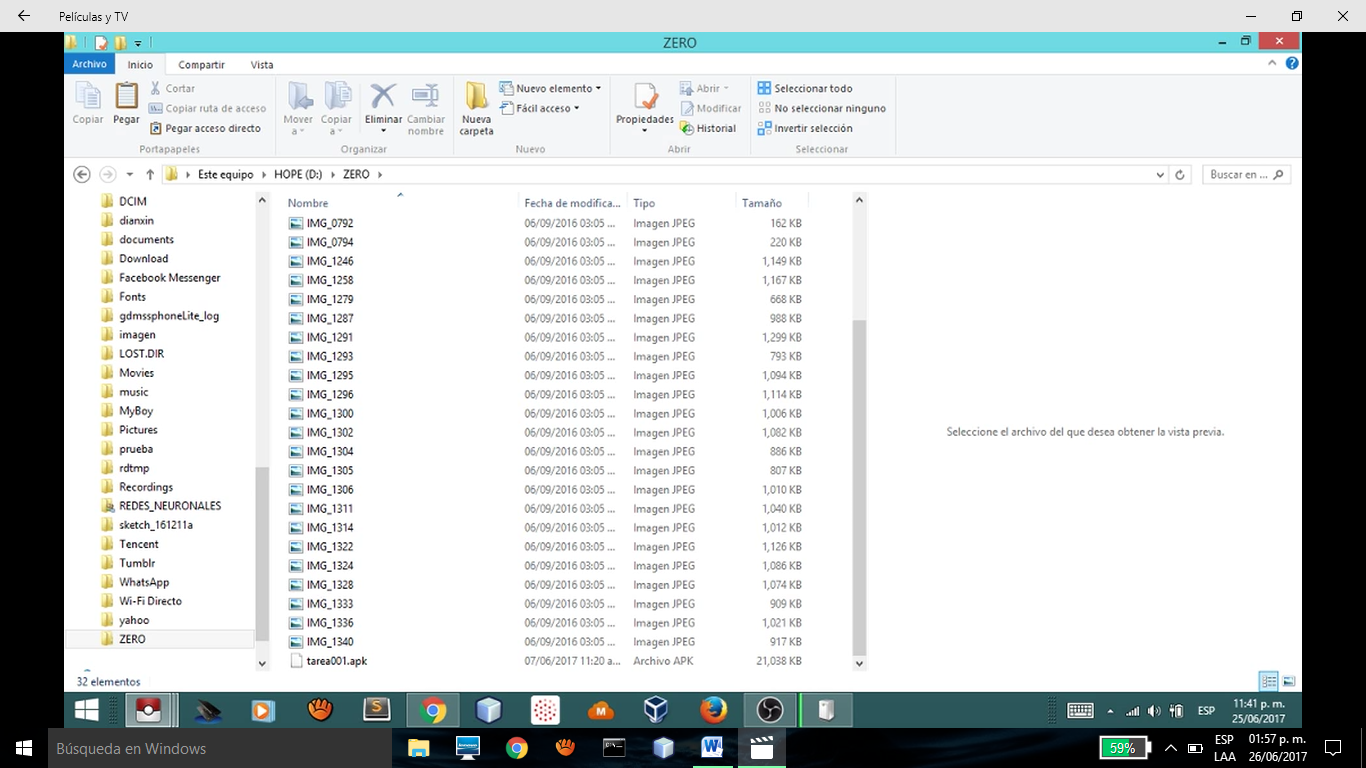
\includegraphics[width=\linewidth]{image/IU33}
  \end{itemize}
\end{frame}

\begin{frame}{34}{Optional Subtitle}
  \begin{itemize}
  \item {
    Vamos a nuestro dispositivo en:
Configuraciones -> Acerca del teléfono
  }
  
 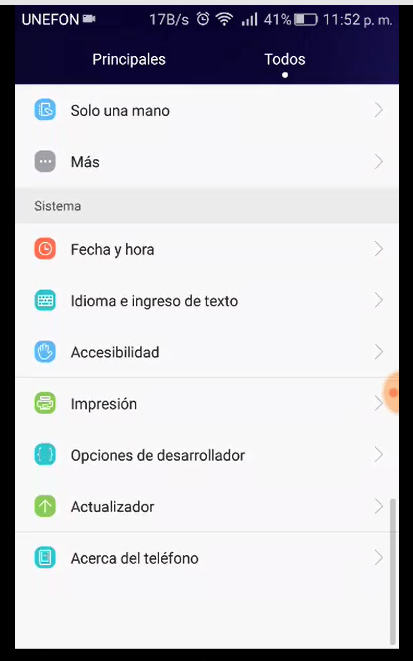
\includegraphics[height=0.7\paperheight]{image/IU34}
  \centering
  \end{itemize}
\end{frame}

\begin{frame}{35}{Optional Subtitle}
  \begin{itemize}
  \item {
    Oprimimos varias veces “Versión del dispositivo” (aprox. 5 veces), hasta que nos diga que tenemos permiso de desarrolladores.
  }
  
  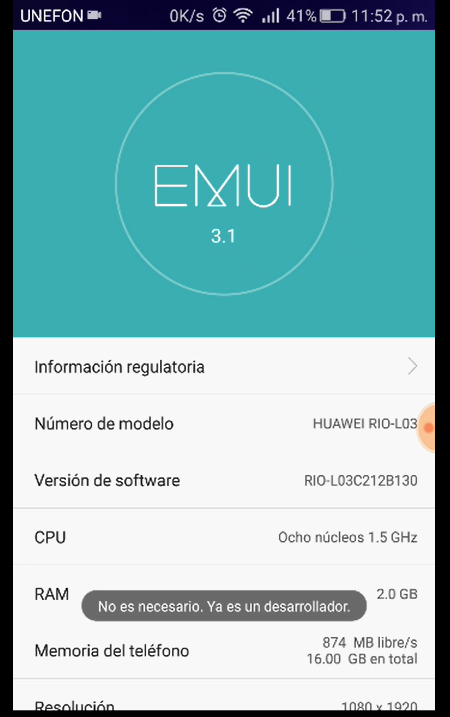
\includegraphics[height=0.6\paperheight]{image/IU35}
  \centering
  \end{itemize}
\end{frame}

\begin{frame}{36}{Optional Subtitle}
  \begin{itemize}
  \item {
    Nos dirigimos a donde guardamos nuestro APK y seleccionamos
  }
  
  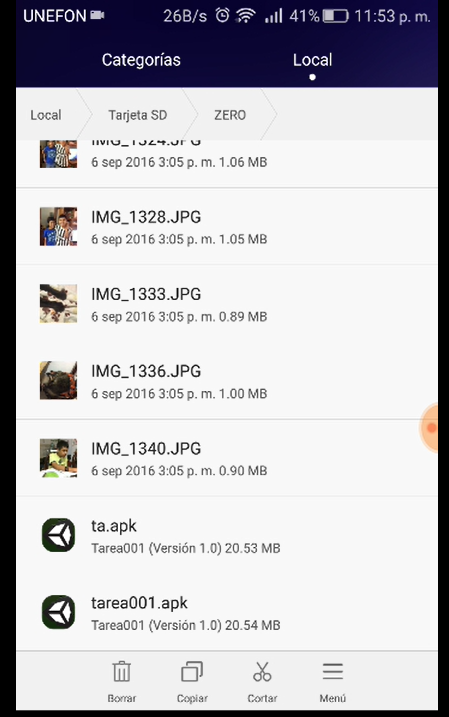
\includegraphics[height=0.7\paperheight]{image/IU36}
  \centering
  \end{itemize}
\end{frame}

\begin{frame}{37}{Optional Subtitle}
  \begin{itemize}
  \item {
    Instalamos
  }
  
  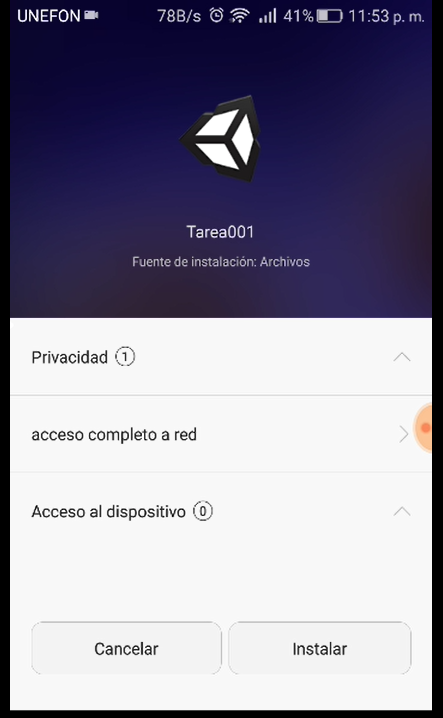
\includegraphics[height=0.7\paperheight]{image/IU37}
  \centering
  \end{itemize}
\end{frame}

\begin{frame}{38}{Optional Subtitle}
  \begin{itemize}
  \item {
   Y abrimos nuestra aplicación
  }
  
\includegraphics[width=\linewidth]{image/IU38}
  \end{itemize}
\end{frame}

\subsection{Unity Remote}

\begin{frame}{01}{Optional Subtitle}
  \begin{itemize}
  \item {
    En el dispositivo Android nos vamos a
    Ajustes -> Opciones de desarrollador
    
  }
  
  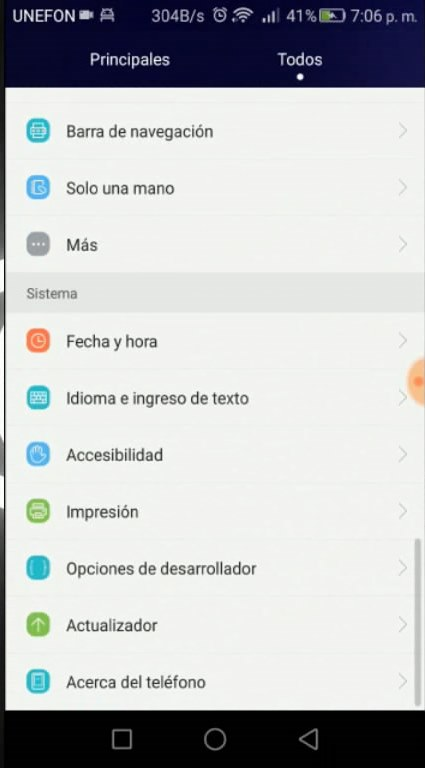
\includegraphics[height=0.7\paperheight]{image2/UR01}
  \centering
  \end{itemize}
\end{frame}

\begin{frame}{02}{Optional Subtitle}
  \begin{itemize}
  \item {
    Activamos la opción de "Depuración USB"
  }
  
  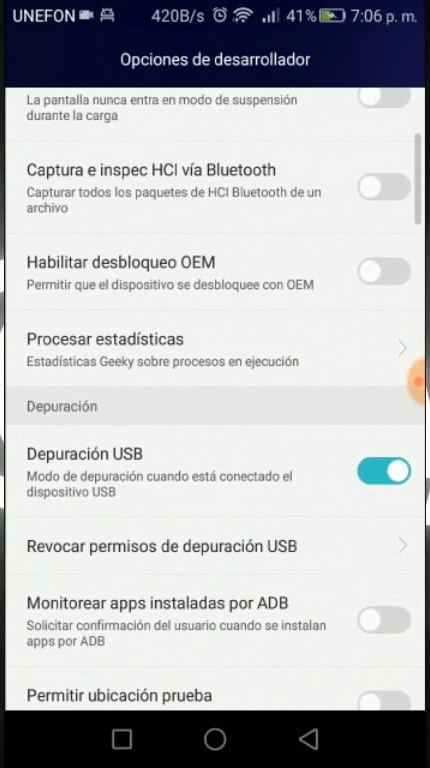
\includegraphics[height=0.7\paperheight]{image2/UR02}
  \centering
  \end{itemize}
\end{frame}

\begin{frame}{03}{Optional Subtitle}
  \begin{itemize}
  \item {
    En el programa de Unity abrimos
    Edit -> Project Settings -> Editor
  }
  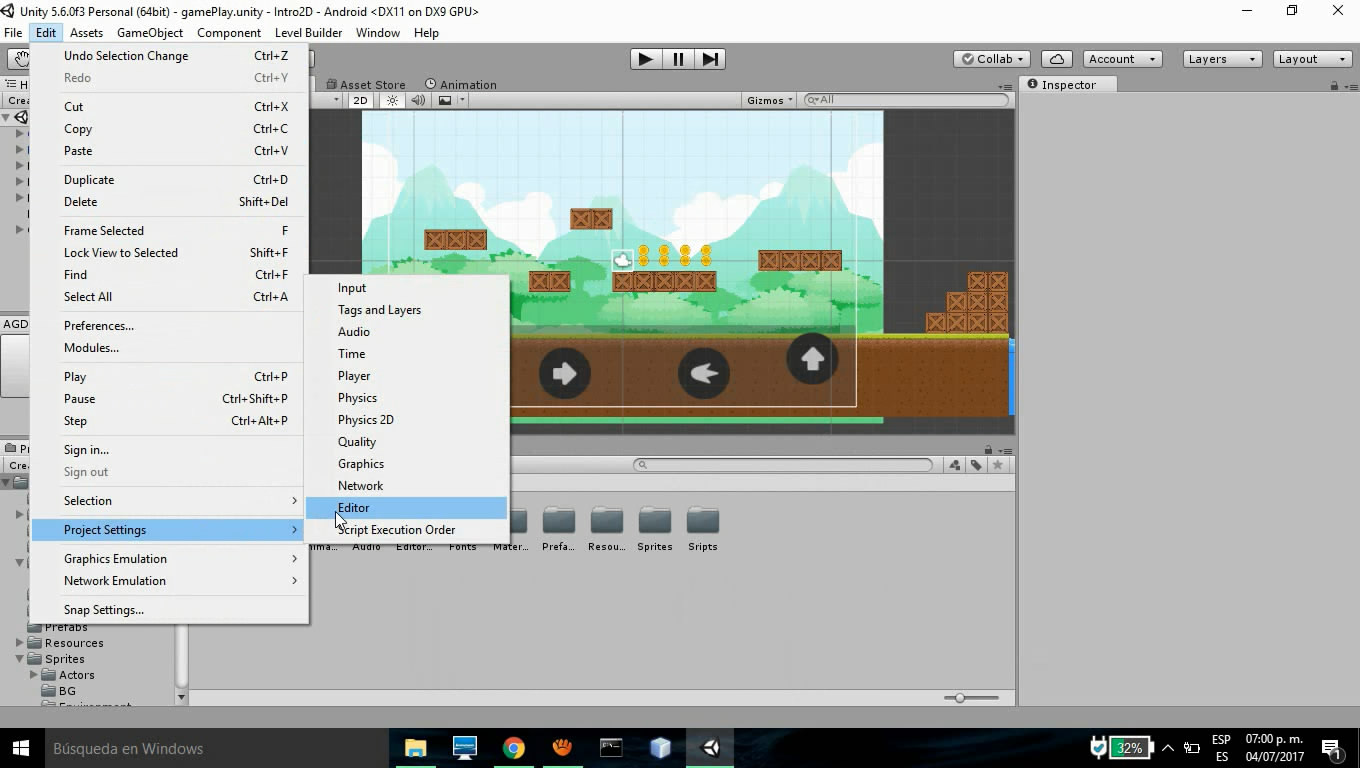
\includegraphics[width=\linewidth]{image2/UR03}
  \end{itemize}
\end{frame}

\begin{frame}{04}{Optional Subtitle}
  \begin{itemize}
  \item {
    En "Editor Settings" dentro de "Device" seleccionamos la opción "Any Android Device"
  }
  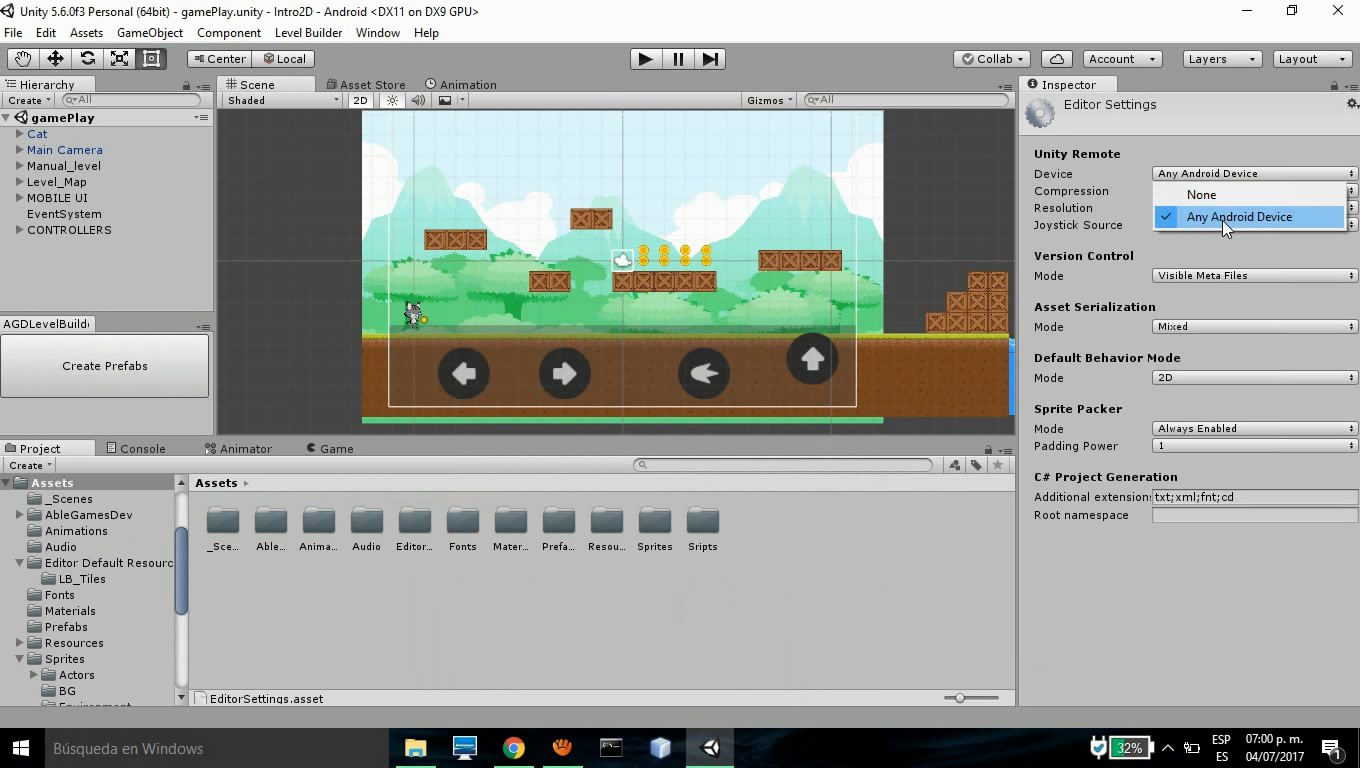
\includegraphics[width=\linewidth]{image2/UR04}
  \end{itemize}
\end{frame}

\begin{frame}{05}{Optional Subtitle}
  \begin{itemize}
  \item {
    En el dispositivo Android descargamos en la "Play Store":
    Unity Remote
  }
  
  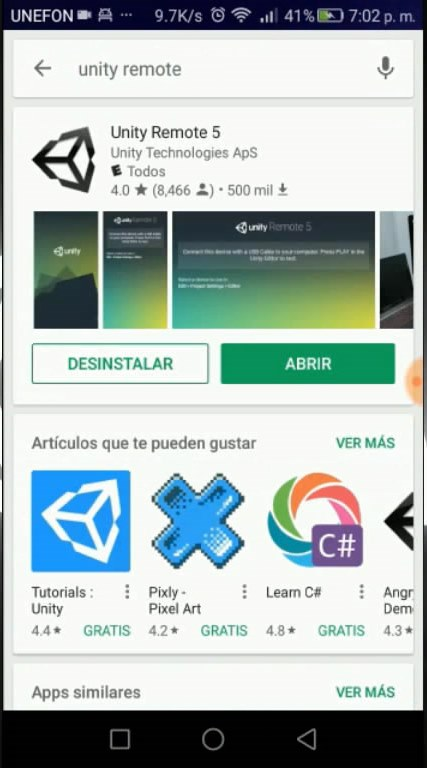
\includegraphics[height=0.7\paperheight]{image2/UR05}
  \centering
  \end{itemize}
\end{frame}

\begin{frame}{06}{Optional Subtitle}
  \begin{itemize}
  \item {
    Abrimos el programa "Unity Remote" y conectamos con un cable USB el dispositivo y la computadora con el proyecto abierto a probar
  }
  
  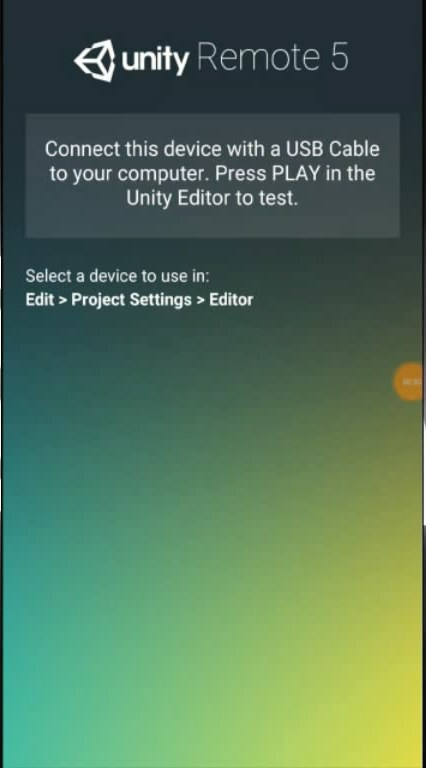
\includegraphics[height=0.6\paperheight]{image2/UR06}
  \centering
  \end{itemize}
\end{frame}

\begin{frame}{07}{Optional Subtitle}
  \begin{itemize}
  \item {
    Oprimimos el ícono de "Play" del proyecto 
  }
  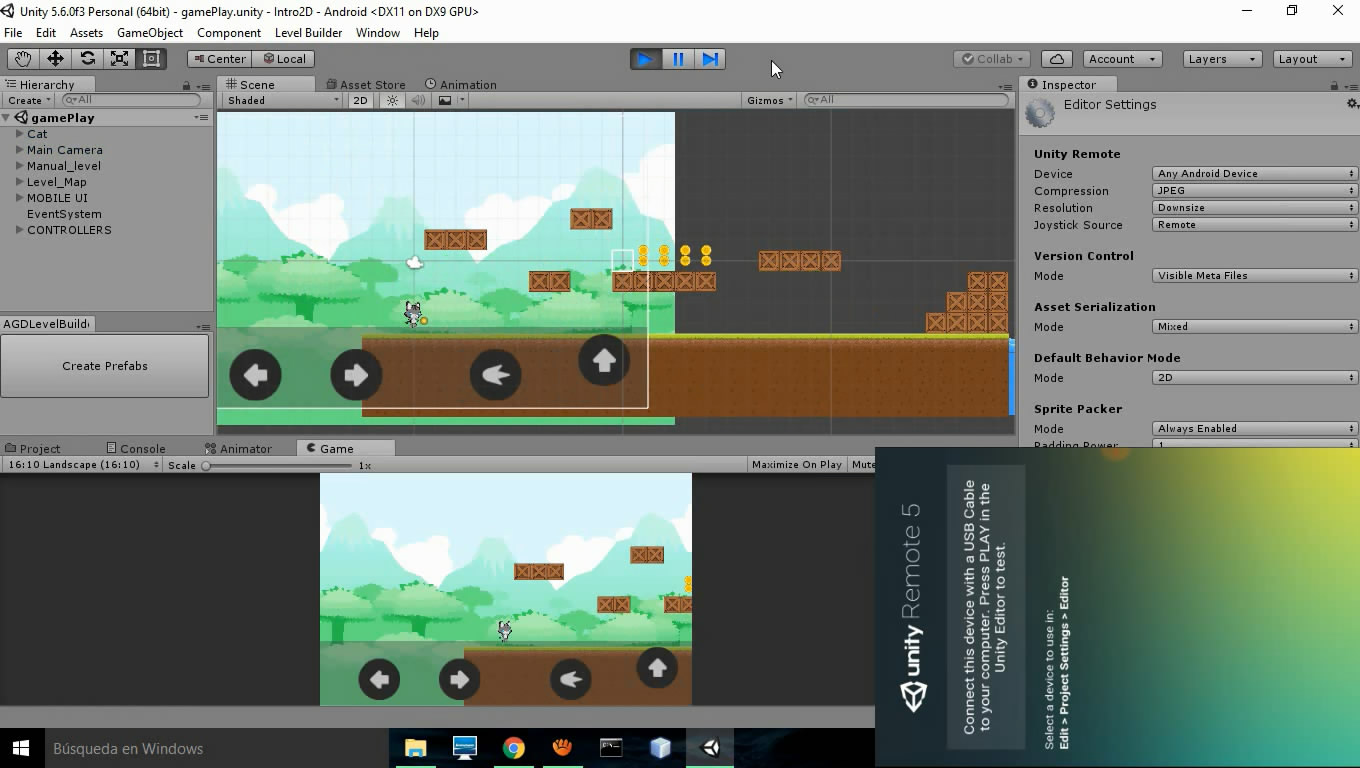
\includegraphics[width=\linewidth]{image2/UR07}
  \end{itemize}
\end{frame}

\begin{frame}{08}{Optional Subtitle}
  \begin{itemize}
  \item {
    Y automáticamente el proyecto a probar se sincronizará en el dispositivo Android
  }
  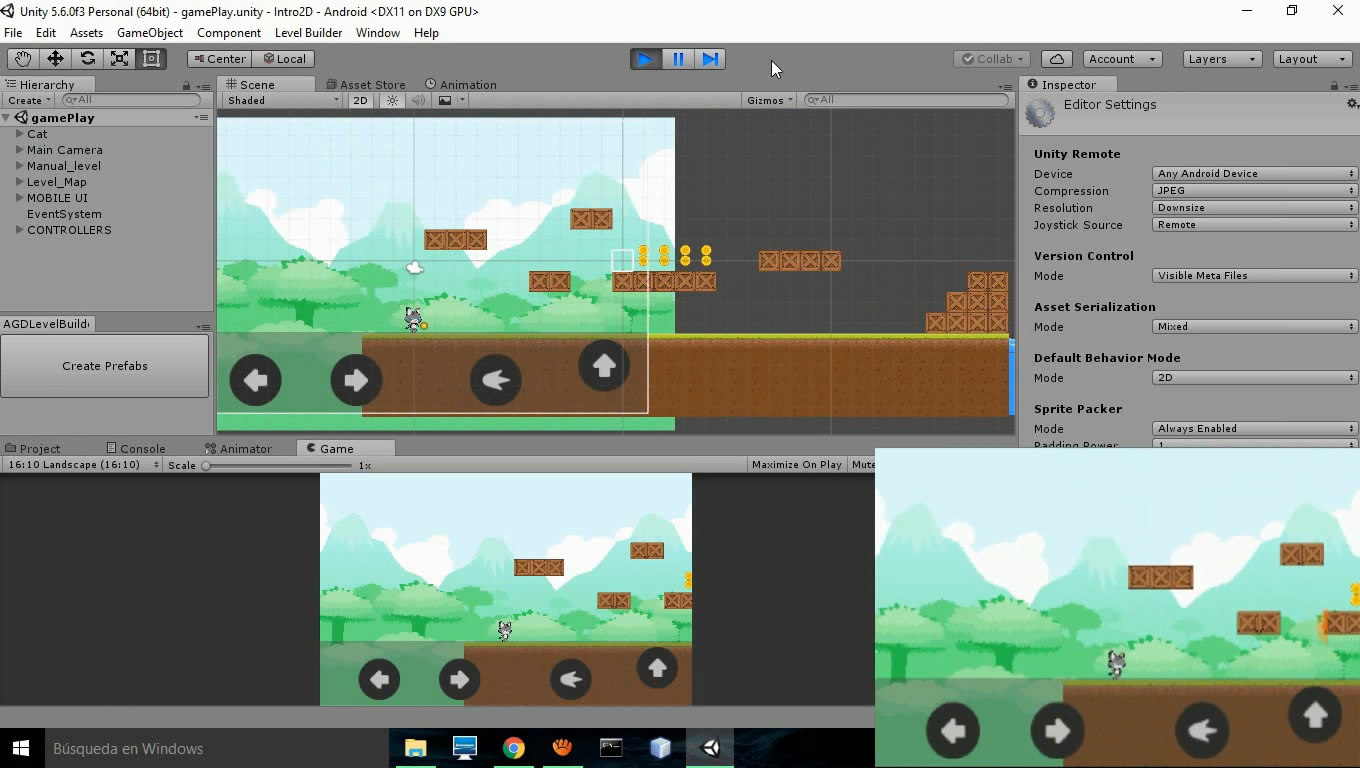
\includegraphics[width=\linewidth]{image2/UR08}
  \end{itemize}
\end{frame}

\begin{frame}{Blocks}
\begin{block}{Block Title}
You can also highlight sections of your presentation in a block, with it's own title
\end{block}
\begin{theorem}
There are separate environments for theorems, examples, definitions and proofs.
\end{theorem}
\begin{example}
Here is an example of an example block.
\end{example}
\end{frame}

% Placing a * after \section means it will not show in the
% outline or table of contents.
\section*{Summary}

\begin{frame}{Summary}
  \begin{itemize}
  \item
    The \alert{first main message} of your talk in one or two lines.
  \item
    The \alert{second main message} of your talk in one or two lines.
  \item
    Perhaps a \alert{third message}, but not more than that.
  \end{itemize}
  
  \begin{itemize}
  \item
    Outlook
    \begin{itemize}
    \item
      Something you haven't solved.
    \item
      Something else you haven't solved.
    \end{itemize}
  \end{itemize}
\end{frame}



% All of the following is optional and typically not needed. 
\appendix
\section<presentation>*{\appendixname}
\subsection<presentation>*{For Further Reading}

\begin{frame}[allowframebreaks]
  \frametitle<presentation>{For Further Reading}
    
  \begin{thebibliography}{10}
    
  \beamertemplatebookbibitems
  % Start with overview books.

  \bibitem{Author1990}
    A.~Author.
    \newblock {\em Handbook of Everything}.
    \newblock Some Press, 1990.
 
    
  \beamertemplatearticlebibitems
  % Followed by interesting articles. Keep the list short. 

  \bibitem{Someone2000}
    S.~Someone.
    \newblock On this and that.
    \newblock {\em Journal of This and That}, 2(1):50--100,
    2000.
  \end{thebibliography}
\end{frame}

\end{document}


